\documentclass[letterpaper,11pt,openany]{book}
\usepackage[centertags]{amsmath}
%\usepackage[pdflatex]{fullbib-bibtex}
\usepackage{graphicx,amsfonts,amssymb,amsthm,newlfont,macros}
\usepackage{tikz}
\usepackage{float}
\usepackage{graphics}
\usepackage{caption}
\usepackage{hyperref}
\usepackage{booktabs}
\usepackage{tabularx}

\usetikzlibrary{shapes.geometric, arrows}

\newcommand\mat[1]{\boldsymbol{#1}}
\newcommand\vect[1]{\boldsymbol{#1}}
\newcommand\eul{\textup{e}}
\newcommand\imag{\textup{i}}
\makeatletter
% Don't think these are needed so commented them out
%\let\@vwritefile\@writefile
%\def\@ADL@backpage#1{\trelax}
%\newif\ifmtcsecondpart
\@input{classical-control.bux}
\makeatother
\title{MTHE 430 Lab Manual}
\date{\today}
\sloppy 
\begin{document}
\maketitle
\tableofcontents

\chapter{Feedback and PID control}

In this lab you will be examining the effects of feedback on system
performance.  In particular, you will design a control, \(R_{C}\), for the
motor using the principles of PID control as shown in Figure~\ref{fig:PID}\@.
\begin{figure}[htbp]
    \centering
    \begin{picture}(300,75)
        \put(-1,50){\(\hat\theta_{d}(s)\)}
        \put(22,53){\vector(1,0){13}}
        \put(40,53){\circle{7}}
        \put(47,53){\vector(1,0){13}}
        \put(30,57){+}
        \put(30,43){\_}
        \put(63,37){\framebox(85,33){\normalsize\(P+I \frac{1}{s}+Ds\)}}
        \put(150,53){\vector(1,0){20}}
        \put(175,53){\circle{7}}
        \put(180,53){\vector(1,0){20}}
        \put(203,37){\framebox(42.5,33){\Large\(\frac{k_{E}}{s(s+\frac{1}{\tau})}\)}}
        \put(247,53){\vector(1,0){30}}
        \put(280,50){\(\hat\theta(s)\)}
        \put(259,53){\line(0,-1){45}}
        \put(259,8){\line(-1,0){219}}
        \put(40,8){\vector(0,1){40}}
        \put(180,58){\(\hat u(s)\)}
    \end{picture}
    \caption{PID control system}\label{fig:PID}
\end{figure}%

\section{Key Concepts}
In this lab, you will be implementing a PID controller into a closed loop
system. The main issue with open loop systems is that we only have
control over the reference trajectory, and therefore cannot account for
disturbances. Now, if we were to use feedback, we could attempt to control
the \emph{error} signal, which is the difference between the reference
trajectory (i.e.\ desired angle, or state of the motor) and the measured output.

A goal of a standard PID controller is to  tune the system to behave a certain
way by using various constants to correct the error signal. The three contstants
of a PID controller are \emph{Proportional}, \emph{Integral}, and \emph{Derivative}
controls.
\begin{itemize}
    \item \textbf{Proportional} control acts on the present value of the error signal. This is the most
          dominant of the three terms, but it can also leave some steady state error.
    \item\textbf{Integral} control accounts for the past values of error which is accumulated over time.
          This term will eliminate the steady state error that is left behind by the proportional control
          term, and also reduce rise time.
    \item \textbf{Derivative} control looks at the rate of change in the error signal, and attempts to
          correct for possible future values of error. For example, if the system is rapidly approaching
          its reference trajectory, (i.e.\ the error signal is rapidly approaching zero) the system will be
          able to slow down and avoid overshoot. Derivative control helps improve the settling time and
          stability of the system.
    \item Figure~\ref{fig:PIDExp} illustrates the concepts of a PID controller. You have some error
          signal, where the proportional term acts on the current state of the system, the integral term
          sums up all previous error, and the derivative term attempts to predict and control future error.

          \begin{figure}
              \centering
              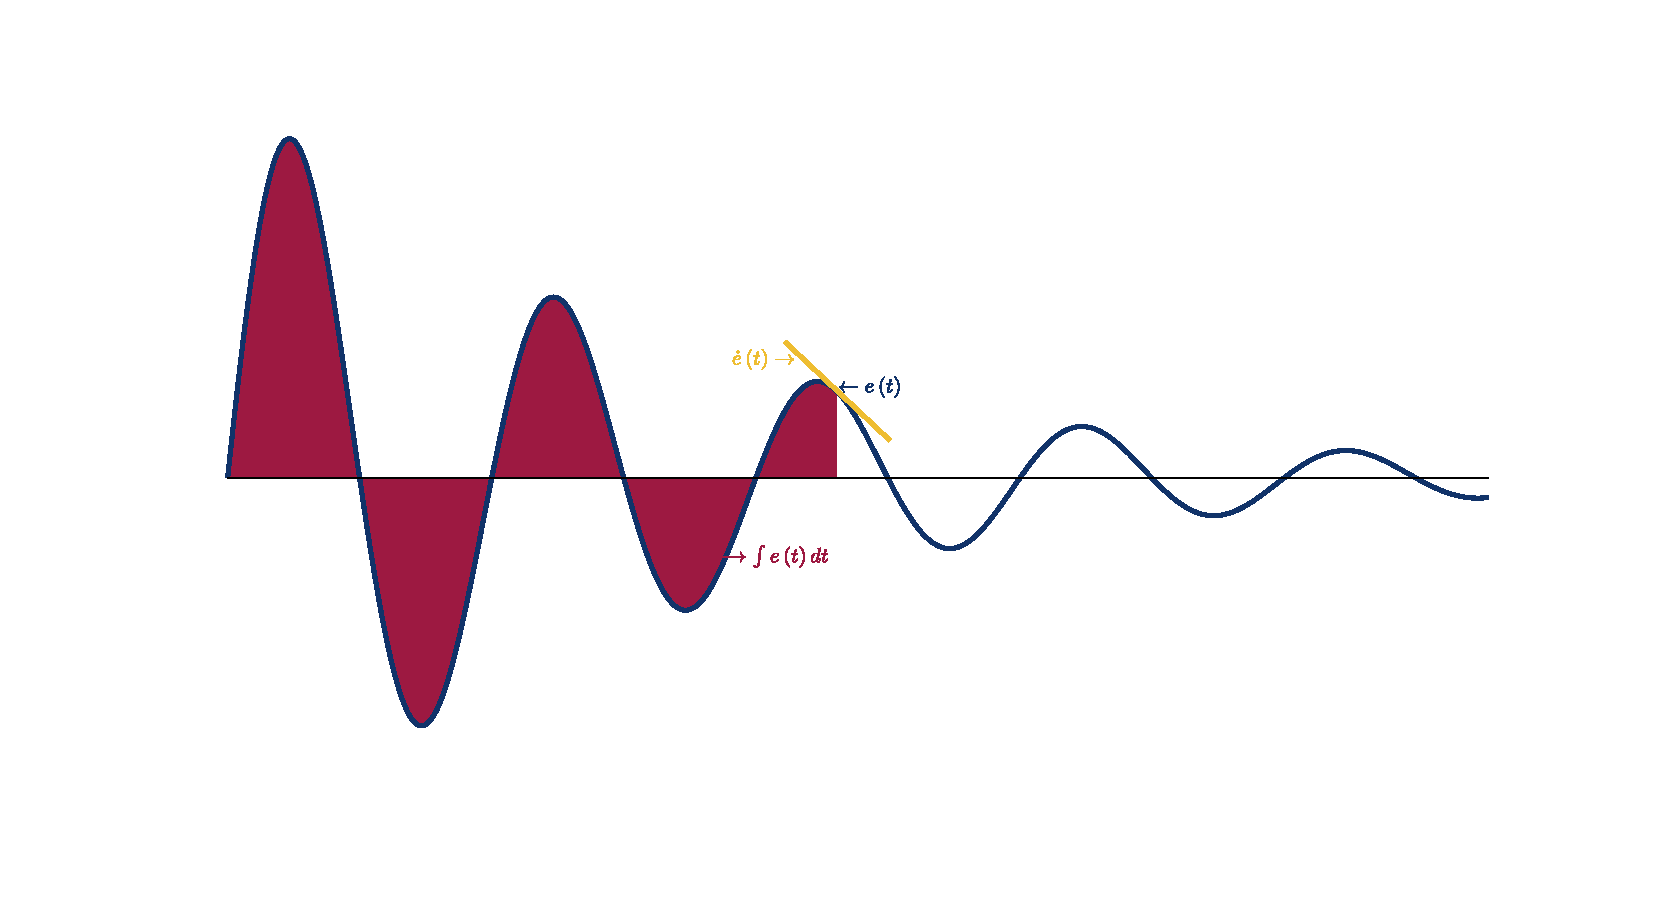
\includegraphics[width = 0.8\hsize]{pix/PIDSchematic.eps}
              \caption{Arbitrary error signal with a PID controller acting on it}\label{fig:PIDExp}
          \end{figure}

\end{itemize}
It is important to remember that when using  PID controllers, there will always be an element of
compromise within your system. For example, the ideal system will have a very low rise time, with
little to no steady state error or settling time, and no overshoot. However, this is very unrealistic in
the real world. If you were designing a highly precise robotic arm, you may need to tune your
controller in a way that there is practically no steady state error, but in order to do so, you will need to
have a higher rise time (i.e.\ the arm will move slowly, but it will go exactly where you need it). On
the other hand, you may have a system that requires a quick reaction time, for which you may need
to accept that there could be overshoot, or some steady state error.

You will also examine the concept of system types and their relation to PID controllers. Essentially,
systems can be type 0, 1, 2, etc \ldots A systems ``type'' determines its ability to track
the error on a given reference trajectory. For example, a system of type \(k \) can track
a reference trajectory with a bounded error for polynomials up to degree \(k \) (See Proposition
8.11 from the course notes for further clarification). We will see how the different terms from the PID controller transfer function affect the system type.

\section{Background Information}

\begin{itemize}
    \item \textcolor{blue}{TODO: Include some stuff from course notes?}
    \item \textcolor{blue}{TODO: Include simulink model rather than have them make it in procedure?}
    \item Learn the definitions for rise time, settling time, overshoot, steady-state value and steady state error.
    \item The closed loop transfer function of the system in \ref{fig:PID} is given by

          \begin{equation*}\label{eq:transfer}
              T(s)= \frac{R_{C}(s)R_{P}(s)}{1+R_{C}(s)R_{P}(s)}
          \end{equation*}

          where \( R_C = P + I\frac{1}{s} + Ds \) is the controller and \( R_P = \frac{\kappa_E}{s(s+\frac{1}{\tau})} \) is the plant. If using P, I, and D controls individually, the

    \item Determine the location of the closed loop poles when using P, I, D controls
          individually. What condition is required on the poles such that the system is BIBO stable?
\end{itemize}

\section{Procedure}

\begin{enumerate}
    \item Prepare a \textsf{Simulink} model to implement a PID controller as
          shown in Figure~\ref{fig:model6}\@. \emph{Modify your model from lab 1 or 2}.
          Figure~\ref{fig:model6}\@.
          \begin{figure}[htbp]
              \centering
              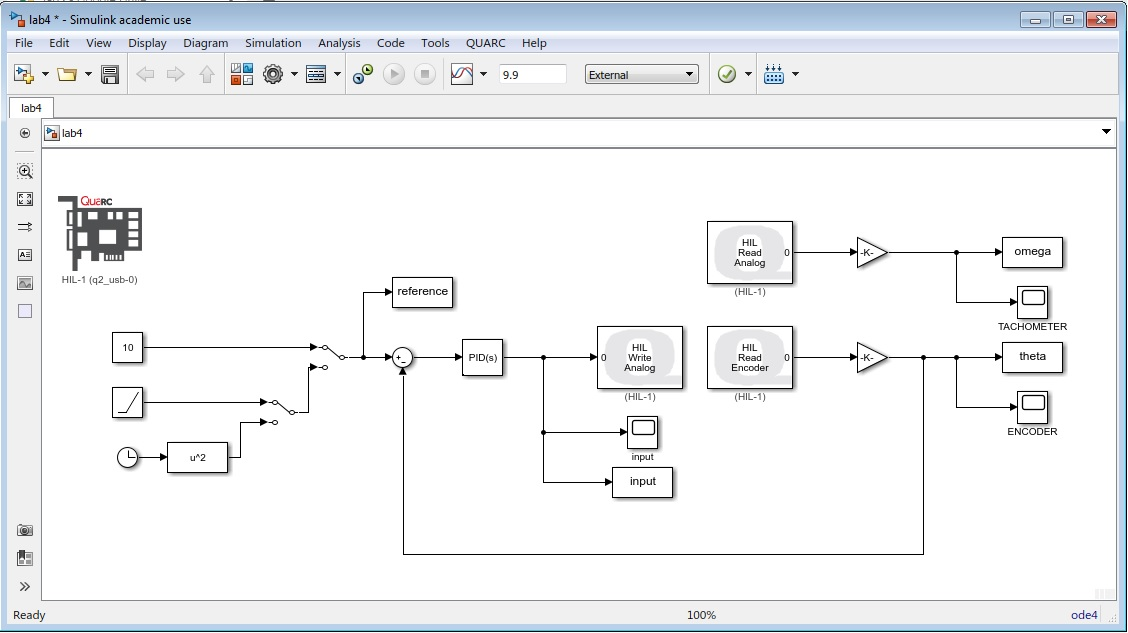
\includegraphics[width=0.6\hsize]{pix/performanceSpecificationModel4.jpg}
              \caption{\textsf{Simulink} model for a DC Servo Motor
                  system}\label{fig:model6}
          \end{figure}%
          The \verb|PID| block can be found in the \verb|Simulink| menu under the
          \verb|Continuous| section parameters.

          As shown in Figure~\ref{fig:PIDparameters}\@,
          \begin{figure}[htbp]
              \centering
              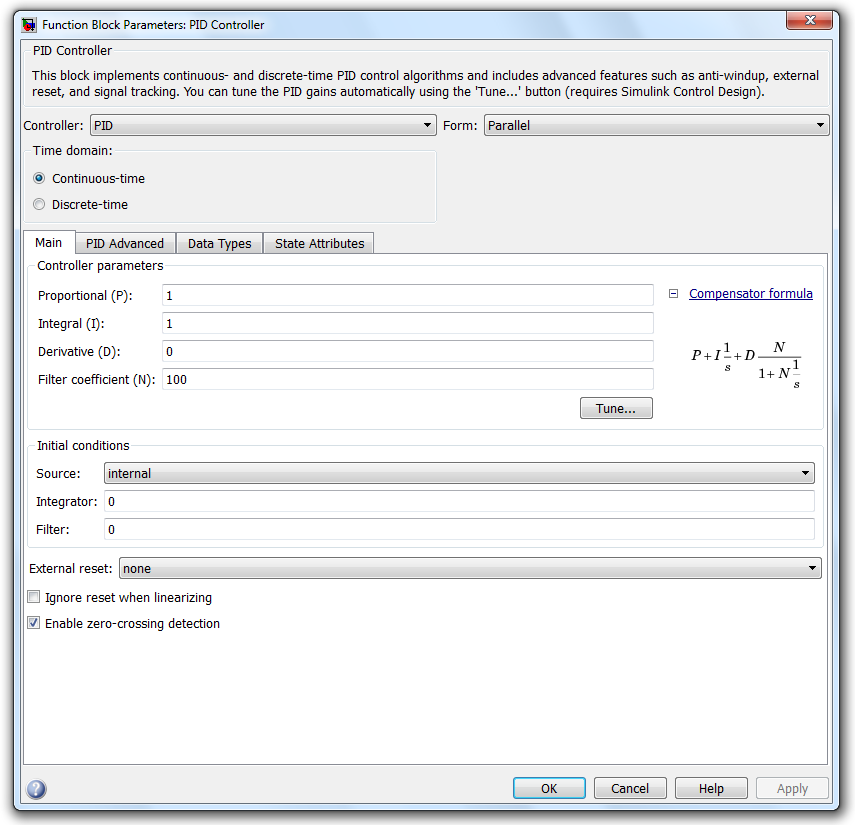
\includegraphics[width=0.6\hsize]{pix/PID.PNG}
              \caption{Screen shot of the \texttt{PID Controller} block}\label{fig:PIDparameters}
          \end{figure}%
          the \verb|PID| block contains three parameters: \(P\) is the proportional gain, of the controller; \(I\) is the integral action parameter which is equal; the \(D\) term provides the derivative action.
    \item\label{step:2} Set the desired angle to 10 radians.  The desired input is entered as
          shown in Figure~\ref{fig:model6} in the \verb|Constant| block. Remember to
          use the appropriate gain values from Table~\ref{tab:conversionFactors} for
          the encoder and tachometer to show results in radians.  Do not forget to
          change the \verb|solver| to \verb|ode 4| in \verb|Configuration Parameters|
          (\verb|Ctrl+E|).

    \item \textbf{Proportional Term}\label{step:3} \begin{enumerate}
              \item Build and run the \textsf{Simulink} model using only the
                    proportional term (i.e., set \(I\) and
                    \(D\) to zero). Comment on the effects of using various values of \(P\).
                    In particular, comment on the overshoot, rise time, settling time, and the
                    steady-state error for different values of \(P\), and be sure to tabulate this data (a table in Excel is an efficient way to do this). Use at least three different values of \(P\).

              \item Keep \(D\) and \(I\) at 0 and increase the value of \(P\) so the
                    system oscillates about the desired value of 10 radians without (seemingly)
                    decreasing in magnitude. Print a copy of the encoder output at that value, and a copy when using a slightly lower value of \(P\).

              \item Now reset your \(P\) value to the ``good'' value (i.e.\ not the value that makes
                    the system oscillate about 10 radians, but the value where you get a ``desirable'' response). Plot the error response of this system (i.e.\ the difference between input and output).
              \item Repeat the previous step but this time replace the constant input with linear input (i.e.\ disconnect the ``10'' block and connect the linear block). Plot the error response.
              \item Repeat the previous step but with the quadratic input (you may have to divide the quadratic term by 2 to prevent the encoder from going out of range).
              \item Based on the above error results, what is the type of the system when using only proportional control?
          \end{enumerate}

    \item \textbf{Derivative Term}\label{step:4} \begin{enumerate}
              \item Test various \(D\) values while keeping \(P\) constant (at the ``good'' value you found in the previous section), and comment on overshoot, rise time, settling time, and steady-state error. Again, tabulate this data, and decide on some ``good'' value of \(D\).
              \item Now, set \(P\) to 0 and repeat steps (c)-(e) from \ref{step:3} using only derivative control.
              \item Based on the above error results, what is the type of the system when using only derivative control?
          \end{enumerate}

    \item \textbf{Integral Term}\label{step:5} \begin{enumerate}
              \item Set your values of \(P\) and \(D\) to the values you found above, and test various \(I\) values.  Comment on the overshoot,
                    rise time, settling time, and steady-state error for these values of
                    \(I\), and tabulate the data.

              \item Now, set \(P\) and
                    \(D\) to zero and repeat steps (c)-(e) from \ref{step:3} using only integral control.
              \item Based on the above error results, what is the type of the system when using only integral control?
          \end{enumerate}

    \item Now we will consider a more complicated function input. To make things interesting, have the desired angle behave
          as four different functions on different intervals.  This can be achieved by
          preparing the \textsf{Simulink} model shown in Figure~\ref{fig:multiSwitch}\@.
          \emph{You do not need to use the exact same functions as shown in the figure}. Pick
          four functions that you think would be interesting.
          \begin{figure}[htbp]
              \centering
              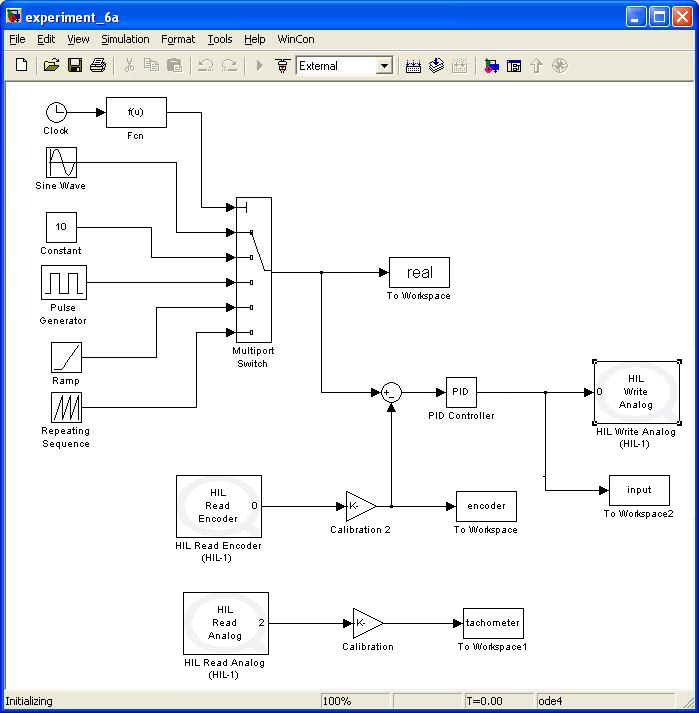
\includegraphics[width=0.6\hsize]{pix/lab6b.jpg}
              \caption{\textsf{Simulink} model for the implementation of multiple inputs and PID control}\label{fig:multiSwitch}
          \end{figure}%
          In this model, a number of possible sources have been introduced along with
          the switching logic.  The switching logic is based on the value of the
          function, \verb|4 sin(0.2*t)^{2}+1|.  This function, although arbitrary,
          assumes a value between 1 and 5 which is associated with ports 1 through 5 of
          the \verb|Multiport Switch| block.  The switching function is entered using
          the \verb|Fcn| block as indicated in Figure~\ref{fig:switchConfig}\@.
          \begin{figure}[htbp]
              \centering
              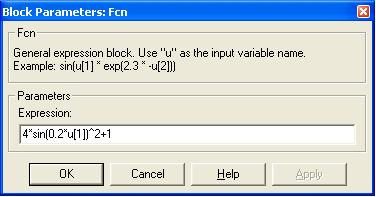
\includegraphics[width=0.6\hsize]{pix/fcnParameters.jpg}
              \caption{Configuration of the \texttt{Fcn} block for the implementation of multiple inputs and PID control}\label{fig:switchConfig}
          \end{figure}%

    \item Run the system and prepare a plot comparing the angle and the desired angle
          trajectory, making sure to note the values of the PID coefficients. You may have to tweak the PID values you found in previous sections in order to get a better trajectory.

          When you have completed the lab, make sure you save your files in the folder
          you created in Lab~\ref{chap:intro}\@.

\end{enumerate}

\section{Deliverables}

Prepare a brief write up describing what you learned from this lab. This does not
need to be a formal report, but all material should be presented in a clear and logical manner,
with concise descriptions where necessary. Include the following / answer the following questions:
\begin{enumerate}
    \item Include tabulated data of the response characteristics from steps~\ref{step:3}, \ref{step:4}, and~\ref{step:5}. Be sure that you are using your ``good'' \(P\) value (i.e. NOT the value that makes the system oscillate about 10 rad / s) when collecting data for \(I\) and \(D\) tests.
    \item Comment on how varying \(P\), \(I\), and \(D\) values impact response characteristics (i.e.\ rise time, settling time, etc\ldots).
    \item Include the plot of the output that oscillates consistently about the reference trajectory of 10 radians
          generated in step~\ref{step:3}. Why do higher \(P\) values increase the oscillation of the output? What is
          happening to the location of the closed loop poles in equation~\eqref{eq:transfer}?
    \item Include the plots of the error response when using only proportional, derivative, or integral control. Using your plots, what is the system type in each case? Is this consistent with the BIBO stability criteria in~\eqref{eq:transfer}?
    \item Include a plot of the output using your PID controller when the desired angle is generated by the multi-input
          switch. Be sure to specify your final P, I, and D values.
\end{enumerate}

%%% Local Variables: 
%%% mode: latex
%%% TeX-master: "lab-manual"
%%% End: 

\chapter{Performance Specifications}

The purpose of this lab is to give you an understanding of the performance of
a second-order system.  In particular, you will be examining the effects that
system parameters have on various features of the output of that system.  In
the second part of the lab, you will examine the disturbance type of several
systems.

\section{Prelab}

Before you go into the lab, you should read the following:
\begin{itemize}
\item Sections 8.2.2, 8.2.3, and 8.3.1 in the course notes on performance specifications.
\item Be sure to familiarize yourself with the concept of system types. 
\end{itemize}
Then, determine the state space representation
$(\mat{A},\vect{b},\vect{c}^{t},\mat{D})$ of the generic second order model:
\begin{equation*}
\ddot y +2\zeta\omega_{0}\dot y+\omega_{0}^{2}y=\omega_{0}^{2}u.
\end{equation*}
Next, solve the above differential equation with a step response ($u = 1$), 
and comment on the effect of $\zeta$ and $\omega_0$, and how this relates to 
the location of the poles of your transfer function. 

\section{Key Concepts}

\begin{enumerate}
\item The main idea behind this lab is to understand how the addition of a zero 
affects the response of a system. For your system, let's say you add a zero at the 
point $\alpha$. What this will do to your governing equation is add a scaled derivative 
of the step response. The derivative of the step response (i.e. the impulse response)  
will be scaled by a factor of $\frac{\omega_0}{\alpha}$. Thus, for very large alpha, 
this term will have little impact on the systems response. However, if this zero exists 
very close to the imaginary axis, your system will have what is called undershoot.
\item Secondly, you must understand the definition of system types. Essentially, 
systems can be type 0, 1, 2, etc... A systems ``type" determines its ability to track 
the error on a given reference trajectory. For example, a system of type $k$ can track 
a reference trajectory with a bounded error for polynomials up to degree $k$. See Proposition 
8.11 from the course notes for further clarification. 


\end{enumerate}

\section{Procedure}

\subsection{Simulation of a second-order system}\label{subsec:simulation}

The model we will be examining is the generic second-order equation, where
the output of the system is position:
\begin{equation}\label{eq:sys}
\ddot y +2\zeta\omega_{0}\dot y+\omega_{0}^{2}y = \omega_{0}^{2}u.
\end{equation}
Since the physical constants of our friendly motor system cannot be changed
in the simple open-loop configuration, we are confined to the world of
simulations.  We will examine the behaviour of the second-order system in
\textsf{Simulink}.
\begin{enumerate}
\item Find the poles of your generic second-order system (or eigenvalues of your $\mat{A}$ matrix).
\item Open \textsf{Matlab} and build a \textsf{Simulink} model according to
Figure~\ref{fig:model7}\@.
\begin{figure}[htbp]
\centering
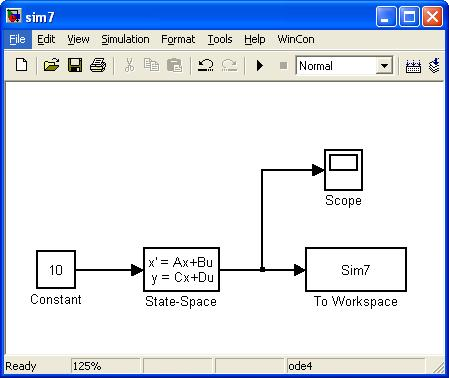
\includegraphics[width=0.6\hsize]{pix/model7.jpg}
\caption{\textsf{Simulink} model for a generic second-order system}\label{fig:model7}
\end{figure}%
You should have determined the values for
$(\mat{A},\vect{b},\vect{c}^{t},\mat{D})$ in your prelab. Define these matrices, in terms of $\zeta$ and $\omega_{0}$, in a script and simply call them in your model. We will use this model in section \ref{NMP}.

\item Run the system in simulation with initial values of $\zeta=0.5$ and
$\omega_{0}=1$\@. As this is a simulation, you do not need to build your system.

\item Using the \verb|step()| function in Matlab (and a \verb|for| loop), plot several values of $\zeta$ on the same graph using your $(\mat{A},\vect{b},\vect{c}^{t},\mat{D})$ matrices.
Print out the graph and write down your observations related to the response characteristics. It may be helpful to use different style of
lines for various values of $\zeta$. Details on plotting with various line
styles are discussed in Appendix~\ref{chap:MATLAB}\@.

\item Repeat the previous step with various values of $\omega_{0}$\@.
\end{enumerate}

\subsection{Non-minimum phase systems} \label{NMP}

The system described in Section~\ref{subsec:simulation} has the transfer
function
\begin{equation*}
T(s)=\frac{\omega_{0}^{2}}{s^{2}+2\zeta\omega_{0}s+\omega_{0}^{2}}.
\end{equation*}
We add a zero to the system as follows:
\begin{equation*}
T(s)=\frac{\hat y(s)}{\hat u(s)}=
\frac{\omega_{0}^{2}}{s^{2}+2\zeta\omega_{0}s+
\omega_{0}^{2}}\frac{(s+\alpha)}{\alpha}.
\end{equation*}
We use the parameter $\alpha$ to vary the position of the zero.  In
particular, we can use it to place our zero in $\mathbb{R}_{<0}$ or
$\mathbb{R}_{>0}$\@.  Notice that we have $\alpha$ in the denominator as
well.  This is a done to normalize the system at $s=0$\@.

To convert this back into the time domain, we simply cross-multiply the
transfer function to get the state equation
\begin{equation*}
\ddot y +2\zeta\omega_{0}\dot y+\omega_{0}^{2}y =
\frac{\omega_{0}^{2}}{\alpha}\dot u+\omega_{0}^{2}u.
\end{equation*}
You can see that the only difference is that we now have a term involving
$\dot u$.  Since $u$ is a step function, $\dot u$ is going to be an impulse
function.\footnote{The derivative here is understood in the sense of
distributions.}  Implementing an impulse function cannot be done directly,
but we can side-step the problem by cooking the initial conditions so that
our initial value problem is a solution to our system when given a step
input.  It turns out that these initial conditions are $y(0)=0$, and $\dot
y(0)=\frac{\omega_{0}^{2}}{\alpha}$\@.\footnote{This is a little involved,
but see Section 3.6.5 of the course text for
details.}
\begin{enumerate}
\item Modify the model from the previous section to incorporate the zero
added to the system by adding the initial conditions. The way to enter
initial conditions into the model is shown in
Lab~\ref{chap:controlandobserve}\@.

\item For $\alpha = \left\{0.1, 1, 10\right\}$, what is the effect of increasing
$\alpha$ on the rise time, settling time, overshoot, and peak
time?  Using \textsf{Matlab}, plot the output of these positive
$\alpha$ values and print the graph.  On the graph, write down your
discoveries. \label{step1}

\item For $\alpha = \left\{-0.1, -1, -10\right\}$, what is the effect of increasing the
magnitude of $\alpha$ on the rise time, settling time, overshoot,
and peak time? Using \textsf{Matlab}, plot the output of these negative $\alpha$ values and print the graph.  On the graph, write down
your discoveries.  What is the most noticeable characteristic of a
non-minimum phase system?  \label{step2}
\item\label{step:superposition} Lastly, we will be observing exactly what the addition of a zero does 
to the system. 
\begin{enumerate}
\item In Matlab, plot the step response and impulse response of your 
original system (without the zero) shown in equation~\ref{eq:sys} using the \verb|step| and 
\verb|impulse| commands. 
\item \label{step3} On a separate graph, plot the addition of the step response with 
the impulse response scaled by a factor of $\frac{\omega_0^2}{\alpha}$ (use the same $\alpha$ values from above). Note: only the impulse response should be scaled. When using the 
\verb|step| and \verb|impulse| commands, you must ensure that the arrays have the same length in 
order to superimpose them. This may involve truncating one array to match the length of the other. 
\item Comment on your plots obtained in part \ref{step3} with those obtained in step \ref{step1} and \ref{step2}. Hint: The plots should be the exact same. Comment on why that is.
\end{enumerate}
\end{enumerate}

\subsection{System type}

We will now examine three different motor system and the system type of each
one.  The basic configuration is shown in
Figure~\ref{fig:feebackWithDisturbance}\@.
\begin{figure}[htbp]
\centering
\begin{picture}(240,75)
\put(0,50){\(\hat\theta_{d}(s)\)}
\put(20,53){\vector(1,0){15}}
\put(40,53){\circle{7}}
\put(45,53){\vector(1,0){15}}
\put(63,37){\framebox(35,33){$R_{C}(s)$}}
\put(100,53){\vector(1,0){20}}
\put(123,37){\framebox(80,33){$R_{P}(s)=\frac{k_{E}}{s(s+\frac{1}{\tau})}$}}
\put(205,53){\vector(1,0){30}}
\put(237,50){$\hat\theta(s)$}
\put(215,53){\line(0,-1){45}}
\put(215,8){\line(-1,0){175}}
\put(40,8){\vector(0,1){40}}
\put(30,48){\line (1,0) {4}}
\end{picture}
\caption{Feedback system with disturbance}\label{fig:feebackWithDisturbance}
\end{figure}%
This is an interconnected system, but we will take a ``black box'' approach,
applying the disturbance at the input node, and measuring at the output node.
Recall that the motor is modelled by transfer function
$\frac{k_{E}}{s(s+\frac{1}{\tau})}$ when the output is the motor angle
$\theta$\@.
\begin{enumerate}
\item System 1 has the controller transfer function $R_{C}(s)=5$\@.
Verify by hand that the transfer function
\begin{equation*}
T(s)= \frac{R_{C}(s)R_{P}(s)}{1+R_{C}(s)R_{P}(s)}
\end{equation*}
is BIBO stable. Hint: What is $R_{C} = 5$ equivalent to? What do we know about this from lab 3?

\item Determine the system type for this particular system.

\item Assemble (or modify an existing) a \textsf{Simulink} model according to
Figure~\ref{fig:model7a}\@.
\begin{figure}[htbp]
\centering
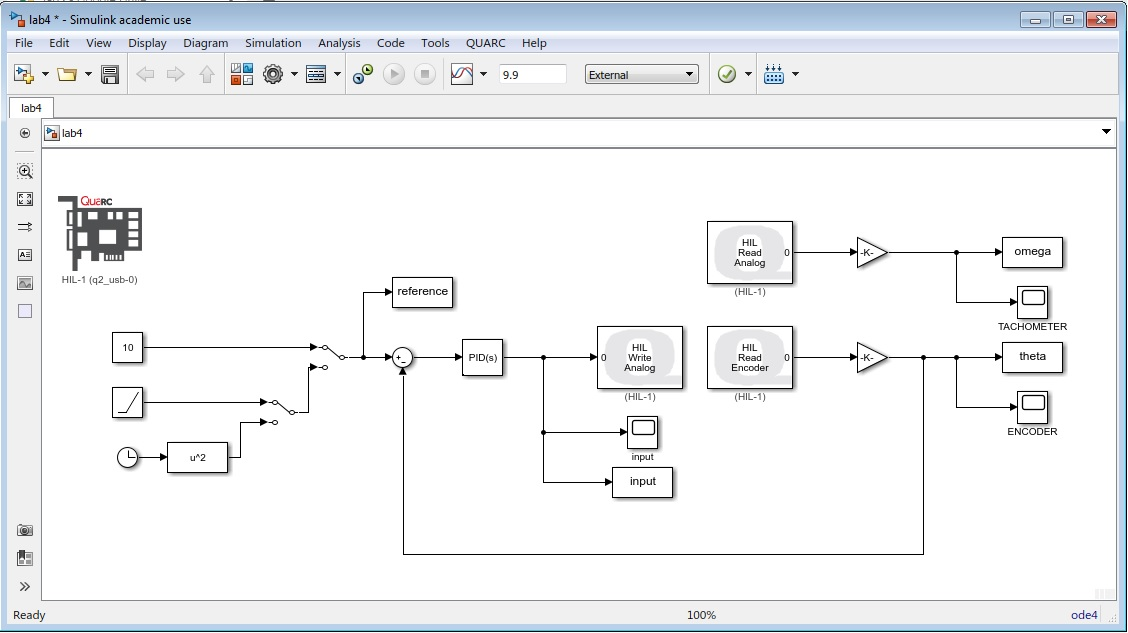
\includegraphics[width=0.6\hsize]{pix/performanceSpecificationModel4.jpg}
\caption{\textsf{Simulink} model for a DC Servo Motor
system}\label{fig:model7a}
\end{figure}%

\item Run the system using the constant input.  What is the steady-state
error of the system?  Plot the error response in \textsf{Matlab} and print a
copy of the plot with appropriate titles and axis labels. Is this consistent
with your earlier work?

\item Repeat the above step, but use a linear and quadratic term (divide the quadratic term by 2 to ensure the encoder does not go out of range) for the
reference signal.  Plot all the error responses and make print outs.  Make
sure you have proper axis labels and titles.

\item System 2 has the same plant transfer function and a new
controller transfer function given by $R_{C}(s)=\frac{1}{s}$\@.  Is this
system BIBO stable?  If so, what is the system type?

\item Make changes to the system to implement the new controller and run the
system with a constant, a linear, and a quadratic reference signal.  Are the
results consistent with your answer from above?

\item System 3 has the same plant transfer function and a new
controller transfer function given by $R_{C}(s)=s$\@.  Is this system BIBO
stable?  If so, what is the system type?

\item Make changes to the system to implement the new controller and run the
system with a constant, a linear, and a quadratic reference signal.  Are the
results consistent with your answer from above? 

\item Plot all the error responses in \textsf{Matlab} graph and print them.
Make sure you have proper axis labels and titles.
\end{enumerate}

When you have completed the lab, make sure you save your files in the folder
you created in Lab~\ref{chap:intro}\@.

\section{Deliverables}

Prepare a brief write up describing what you learned from this lab. This does not
need to be a formal report, but all material should be presented in a clear and logical manner,
with concise descriptions where necessary. Include the following/Answer the following questions:
\begin{enumerate}
\item Include plots of the systems response with varying $\zeta$ and $\omega_0$ values, comment 
on the effect off varying these constants. 
\item For both positive and negative $\alpha$ values, what is the effect of increasing the magnitude 
of $\alpha$ on the rise time, settling time, overshoot/undershoot, and peak time? Include plots. 
\item In step~\ref{step:superposition} of the non-minimum phase system section, explain why your two 
plots are the same. 
\item Create the following table for the system type section. Be sure to include and reference all 
necessary plots for the justification section. 
\begin{table}[htbp]\label{tab:systype}
\centering
\begin{tabular}{|c|p{2.5cm}|p{2.5cm}|p{2.5cm}|c|c|}\hline
System No.&Response to Constant Input&Response to Ramp Input&Response to Quadratic Input&
Type?&Justification\\\hline
System 1&&&&&\\\hline
System 2&&&&&\\\hline
System 3&&&&&\\
\hline
\end{tabular}
\end{table}%
\end{enumerate}

%%% Local Variables: 
%%% mode: latex
%%% TeX-master: "lab-manual"
%%% End: 

\chapter{The Nyquist criterion}

In this lab, you will use the Nyquist contour to determine if a system is
IBIBO stable.  The Nyquist plot is a conformal mapping of a closed loop in
complex plane and it is a tool for the understanding of the stability of a
closed-looped system.  Furthermore, you will be examining the relationship
between the Nyquist contour and the Bode plot, thus familiarizing yourself
with such terms as \emph{crossover frequency}\@, \emph{gain margin}\@, and
\emph{phase margin}\@.

\section{Background Info}
\textcolor{blue}{This references the Bode plots from 393, should we include Bode plots here?}

\section{Procedure}

\subsection{Using the Bode plot to sketch the Nyquist
    contour}\label{sec:bodeNyquist}

For this part of the lab, we will be using the motor in the unity gain
feedback configuration shown in Figure~\ref{fig:generic}\@.
\begin{figure}[htbp]
    \centering
    \begin{picture}(230,75)
        \put(0,50){\(\hat\theta_{d}(s)\)}
        \put(25,53){\vector(1,0){15}}
        \put(45,53){\circle{7}}
        \put(32,57){+}
        \put(50,53){\vector(1,0){20}}
        \put(73,37){\framebox(35,33){\(R_{C}(s)\)}}
        \put(110,53){\vector(1,0){40}}
        \put(152,37){\framebox(35,33){\(R_{P}(s)\)}}
        \put(190,53){\vector(1,0){30}}
        \put(224,50){\(\hat\theta(s)\)}
        \put(206,53){\line(0,-1){45}}
        \put(205,8){\line(-1,0){160}}
        \put(45,8){\vector(0,1){40}}
        \put(35,48){\line (1,0) {4}}
    \end{picture}
    \caption{Feedback system with disturbance}\label{fig:generic}
\end{figure}%
This setup should be quite familiar to you by now, so you should have a
well-developed intuition concerning the IBIBO stability of such a system.  We
will be taking the output of the system to be the motor velocity, \(\omega \),
so our plant transfer function is \(R_{P}(s)=\frac{k_{E}}{s+\frac{1}{\tau}}\).
In Lab 2 you constructed the Bode plot for this system
experimentally.
\begin{enumerate}
    \item Using the Bode plot from Lab 2, determine the gain
          and phase crossover frequencies, and the phase and gain margins at these
          frequencies; see Section 7.2.2 from the course text.

    \item Using the Bode plot determine the general transfer function, from the
          transfer function sketch the corresponding Nyquist contour.  Looking also at
          the transfer function, determine whether or not the system is IBIBO stable.

    \item Start up \textsf{Matlab} and define \verb|t| to be the transfer
          function of the open-loop motor scheme.  Essentially, we are just setting
          \(R_{C}(s)=1\) to see how motor behaves on its own.

    \item To plot the Nyquist contour, use the \verb|Nyquist| command in
          \textsf{Matlab}.

    \item Is the Nyquist contour consistent with what you know about the IBIBO
          stability of the system?  Comment on both the poles of the transfer function,
          and the zeroes of the characteristic polynomial.
\end{enumerate}

\subsection{Using a proportional controller}

We will now turn our attention to the task of using the Nyquist contour as a
tool in determining what range of values of a proportional controller can
take on in order to make the system IBIBO stable.

The plant transfer function \(R_{C}(s) = K\) will be used in the feedback
configuration depicted in Figure~\ref{fig:generic}\@.  The transfer function
for this system is simply
\begin{equation*}
    T(s)=\frac{KR_{P}(s)}{1+KR_{P}(s)}.
\end{equation*}
What is important to note is that the condition \(KR_{P}(s)=-1\) is equivalent
to the condition \(R_{P}=-\frac{1}{K}\). This seems obvious in itself, but what
this allows you to do is to use the Nyquist contour for \(R_{P}(s)\) on its own
(i.e., with \(K=1\)), and determine where you would like the point
\(\frac{1}{K}\) to be. This allows you to get a lot of mileage out of only one
plot. The alternative is to construct the Nyquist contour for many values of
\(K\), and see if each contour has the required number of encirclements of the
point \(-1+\imag0\).  This may not seem like a bad alternative if you have
access to a computer, but the method of normalizing the proportional gain is
much more efficient.

\begin{enumerate}
    \item In \textsf{Matlab}, define the plant transfer function to be
          \(R_{P}=\frac{s+1}{s(\frac{s}{10}-1)}\).

    \item Produce both the Bode plot and the Nyquist contour.  Take a minute to
          further reaffirm your faith in the relationship between the two.

    \item What are the crossover frequencies, and what are the gain and phase
          margins at these frequencies?

    \item Since our plant transfer function has one pole in the right-half
          complex plane, we require one counterclockwise encirclements of the point
          \(\frac{1}{K}\). Using this information, in which region should we place the
          point \(-\frac{1}{K}\)?

    \item What values of \(K\) satisfy the above requirement?

    \item Repeat the above procedure for the plant transfer function
          \(R_{P}(s)=\frac{1}{s{(s+1)}^{2}}\).  Remember, Nyquist plots always close
          clockwise.
\end{enumerate}

\subsection{The phase margin}

In this part of the lab we will quickly demonstrate the phase margin as it
applies to the Nyquist contour.
\begin{enumerate}
    \item We will use the plant transfer function
          \(R_{P}(s)=\frac{1}{s{(s+1)}^{2}}\).  Produce the Bode plot and the Nyquist
          contour of this system.

    \item Determine how much you have to boost the gain (in decibels) to provide
          a phase margin of \(0^{\circ}\) at a gain cross over frequency of
          \(10^{n}\frac{\textup{rad}}{\textup{sec}}\), \(n\in\mathbb{Z}\).  Will the %chktex 35
          resulting system, with this gain boosted by using a proportional controller,
          be IBIBO stable?

    \item The number you get is a scalar that represents the factor by which you
          can ``stretch'' (or ``shrink'' as the case may be) the Nyquist contour
          towards the point \(-1+\imag0\) and still maintain IBIBO stability (assuming
          the system is stable for \(K=1\), which our system is).  Looking at the Nyquist
          contour, does this scalar quantity seem to make sense?  Is this consistent
          with your work from Section~\ref{sec:bodeNyquist}?
\end{enumerate}

When you have completed the lab, make sure you save your files in the folder
you created in Lab~\ref{chap:intro}\@.

%%% Local Variables: 
%%% mode: latex
%%% TeX-master: "lab-manual"
%%% End: 

\chapter{PID design using frequency response}

In this lab, you will use the Bode plot you produced using the measurements
for the motor to design a PID controller to meet specified performance
criteria.

\section{Prelab}

Before you go into the lab, you should read the following:
\begin{itemize}
    \item Section 12.2 from the course text on using
          frequency response method for controller design.
\end{itemize}
Since \textsf{Simulink} does not allow improper transfer functions, you must
use the \verb|PID| block for the controller in this lab.  Find the
relationships between the constants in equation~\eqref{eqn:con1}
and~\eqref{eqn:con2}\@:
\begin{gather}\label{eqn:con1}
    \frac{K}{s}(1+T_{D}s)(s+\frac{1}{T_{I}}),\\\label{eqn:con2}
    P+\frac{I}{s}+Ds.
\end{gather}

\section{Procedure}

Before we implement the controller, we need to do some paper work to design
it.

\subsection{Design specifications}

You are charged with the designing the controller rational function \(R_{C}\)
in the feed back loop in Figure~\ref{fig:PIDfeedback}\@.
\begin{figure}[htbp]
    \centering
    \begin{picture}(230,75)
        \put(0,50){\(\hat u(s)\)}
        \put(20,53){\vector(1,0){15}}
        \put(40,53){\circle{7}}
        \put(28,57){+}
        \put(45,53){\vector(1,0){20}}
        \put(68,37){\framebox(35,33){\normalsize \(R_{C}(s)\)}}%-50 in width
        \put(105,53){\vector(1,0){40}}
        \put(147,37){\framebox(35,33){\normalsize \(R_{P}(s)\)}}
        \put(185,53){\vector(1,0){30}}
        \put(217,50){\(\hat y(s)\)}
        \put(201,53){\line(0,-1){45}}
        \put(201,8){\line(-1,0){161}}
        \put(40,8){\vector(0,1){40}}
        \put(30,48){\line (1,0) {4}}
    \end{picture}
    \caption{Feedback system with disturbance}\label{fig:PIDfeedback}
\end{figure}%
The plant transfer function is that for the motor:
\begin{equation*}
    R_{P}(s)=\frac{k_{E}}{s(s+\frac{1}{\tau})},
\end{equation*}
where you have measured the values for \(k_{E}\) and \(\tau \) in Lab~\ref{chap:intro}\@.

You are asked to design a controller so that the closed-loop system has a
phase margin of \(65^{\circ}\) and a crossover frequency as large as possible.
The controller you will use is a PID controller in the form
\begin{equation*}
    R_{C}(s)=\frac{K}{s}(1+T_{D}s)(s+\frac{1}{T_{I}})=
    K(1+\frac{T_{D}}{T_{I}}+T_{D}s+\frac{1}{T_{I}s}).
\end{equation*}

\subsection{The steps in controller design}

We shall lead you by hand through the design process.
\begin{enumerate}
    \item Produce the Bode plot for plant transfer function using
          \textsf{Matlab}.

    \item In the PID controller design, let us decide to fix \(T_{I}=10T_{D}\).
          You are free to change this ratio during the lab if you find it unsuitable.

    \item Also, to start the design process, let us fix the gain \(K\) to 1.  You
          may want to use the \verb|zpk| function in \textsf{Matlab} to define the
          transfer function.

    \item With the above assumptions, is it true that there is a choice for
          \(T_{D}\) for which the closed loop system is IBIBO stable (IBIBO stability can
          be verified either by Nyquist Criterion or Hurwitz Criterion)?  Is it true
          that, no matter what choice one makes for \(T_{D}\), the closed-loop system
          will be IBIBO stable?  Can you spot the features on your Bode and/or Nyquist
          plot which help you answer this question?  How do these play a role in the
          design of the controller?

    \item Based upon the considerations in the previous step, choose a value for
          \(T_{D}\) which meets the design objectives.

    \item Now choose \(K\) to give the crossover frequency.

    \item Make sure the closed-loop system is IBIBO stable using the Nyquist
          criterion.
\end{enumerate}

You now have values for \(K\), \(T_{D}\), and \(T_{I}\) which you will carry
into the rest of the procedure.

\subsection{Executing the design in hardware/software}

Now you will implement your controller in hardware.
\begin{enumerate}
    \item Open \textsf{Matlab} and build a \textsf{Simulink} model according to
          Figure~\ref{fig:model9a}\@.
          \begin{figure}[htbp]
              \centering
              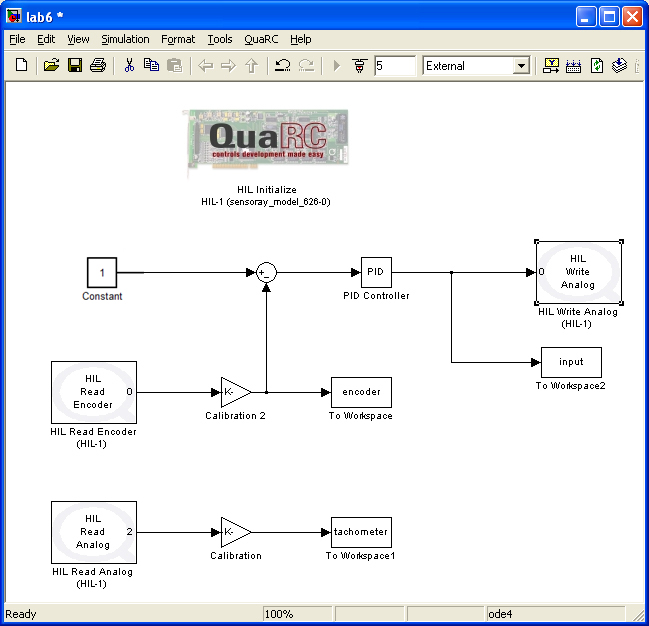
\includegraphics[width=0.6\hsize]{pix/lab9a.jpg}
              \caption{\textsf{Simulink} model for the implementation of PID control using
                  frequency response method; step reference}\label{fig:model9a}
          \end{figure}%

    \item Use values for \(K\), \(T_D\), and \(T_I\) that make the closed loop
          system unstable in hardware.  Use the above contraints you just calculated to
          determine values that cause instability.  Be prepare to shut the system off!
          Produce plots of the unstable system.

    \item Now, using an input step response of \(1\), use the ``good'' values for
          \(K\), \(T_D\), and \(T_I\) to determine the rise time, the percentage
          overshoot, and the \(\epsilon \)-settling time for \(\epsilon=0.5\).

    \item Now run the system with your ``good'' values for \(K\), \(T_D\), and
          \(T_I\) and a sinusoidal input whose magnitude is \(1\) and whose frequency is
          the crossover frequency that was calculated above; see
          Figure~\ref{fig:model9} for the \textsf{Simulink}\@.
          \begin{figure}[htbp]
              \centering
              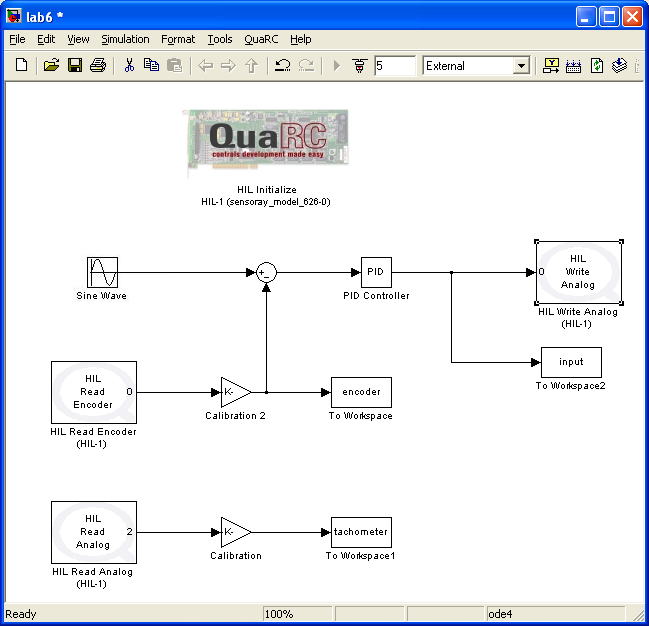
\includegraphics[width=0.6\hsize]{pix/lab9.jpg}
              \caption{\textsf{Simulink} model for the implementation of PID control using
                  frequency response method; sinusoidal reference}\label{fig:model9}
          \end{figure}%
          What is the magnitude of the output compared to the input, and what is the
          phase of the output relative to the input?

    \item Is your controller a good one?  How might you improve it?  What do your
          improvements mean in terms of loopshaping ideas?

    \item Change the ratio of \(\frac{T_{I}}{T_{D}}\) and discuss the effect on the
          performance of the controller.  Does what you observe make sense?  Generate
          plots to demonstrate your observations.
\end{enumerate}

When you have completed the lab, make sure you save your files in the folder
you created in Lab~\ref{chap:intro}\@.

%%% Local Variables: 
%%% mode: latex
%%% TeX-master: "lab-manual"
%%% End: 

\chapter{Controllability and observability}\label{chap:controlandobserve}

This lab will demonstrate the fundamental ideas behind the controllability
and observability properties of a system.  You will analyze a simple circuit
and determine the conditions for observability and controllability.  You will
then proceed to simulate the system using \textsf{Simulink} under various
conditions.

\section{Prelab}

You may wish to read Sections 2.3.1 and 2.3.2 from the
course notes to recall some background on controllability and observability.

Using Figure~\ref{fig:circuit}
\begin{figure}[htbp]
    \centering
    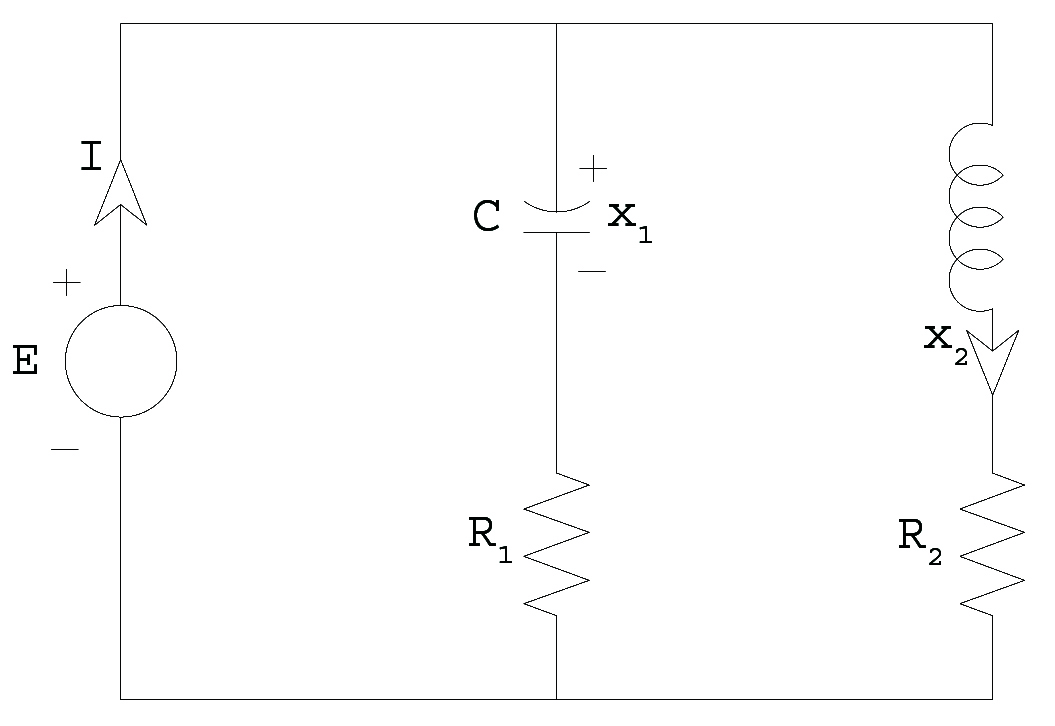
\includegraphics[width=0.6\hsize]{pix/circuitlarge.jpg}
    \caption{State space configuration}\label{fig:circuit}
\end{figure}
as a reference, define \(x_{1}\) as the voltage across the capacitor, and
\(x_{2}\) as the current through the inductor.  Take the output to be the
current entering the circuit, denoted \(I\) in Figure~\ref{fig:circuit}.

\begin{enumerate}
    \item Write out the system equations in the state-space form:
          \begin{eqnarray*}
              \dot{\vect{x}}=\mat{A}\vect{x}+\vect{b}u,\\y=\vect{c}^{t}+\mat{D}u.
          \end{eqnarray*}
          If you are having trouble getting the differential equations, or just not
          ``electrically inclined'', you should review past course notes on electrical
          circuits and differential equations.  Suck it up, Apple Mech students!
          \begin{itemize}
              \item When finding the differential equations for a system, your goal should
                    be to determine an expression for the derivative of each state variable in
                    terms of the state variable(s) and the forcing function.  Once you have %chktex 36
                    these, you can determine \(\mat{A}\) and \(\vect{b}\).

              \item The following facts may be useful.  The current through a capacitor is
                    given by \(I_{c}=C\frac{dV_{C}}{dt}\), the voltage across an inductor is
                    given by \(V_{L}=L\frac{dI_{L}}{dt}\), and the voltage across a resistor is
                    given by Ohm's law, \(V_{R}=I_{R}R\).  By Kirchoff's voltage law, the voltage
                    across each branch of the circuit is simply \(E\). You can use this fact to
                    get expressions for \(\mat{A}\) and \(\vect{b}\).

              \item Since the output is the current entering the circuit, and you will by
                    this point have expressions available for the current in each branch, you can
                    use Kirchoff's current law (i.e., conservation of current) to determine
                    expressions for \(\vect{c}\) and \(\mat{D}\).
          \end{itemize}

    \item Calculate the controllability matrix \(\mat{C}(\mat{A},\vect{b})\).

    \item Calculate the observability matrix \(\mat{O}(\mat{A},\vect{c})\).

    \item Determine the conditions under which the system is uncontrollable.
          Recall that a square matrix has full rank if and only if its determinant is
          non-zero.

    \item Determine the conditions under which the system is unobservable.

    \item When the system is uncontrollable, determine the set of reachable
          points for zero initial conditions.  This is going to be a one-dimensional
          vector space, so there is a simple relationship between \(x_{1}\) and \(x_{2}$.
          Determine this relationship when the system is uncontrollable.

    \item When the system is unobservable, determine the set of initial
          conditions that yield the same output, and the linear relationship between
          the initial conditions.
\end{enumerate}

\section{Procedure}

Via simulation, you will determine the conditions under which the circuit in
Figure~\ref{fig:circuit} is controllable and/or observable.

\subsection{Controllability}

When analyzing the controllability, you will be examining the behaviour of
the system states.  Recall that a rough definition of controllability is:
``starting from the origin, you can reach any point in state space by
applying an appropriate input.''
\begin{enumerate}
    \item Build the \textsf{Simulink} model as shown in
          Figure~\ref{fig:model2}.
          \begin{figure}[htbp]
              \centering
              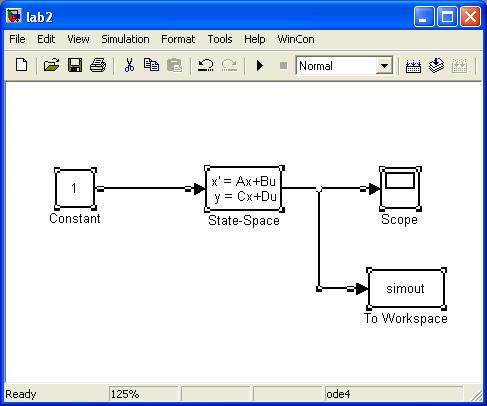
\includegraphics[width=0.6\hsize]{pix/controlandobservemodel.jpg}
              \caption{\textsf{Simulink} model for Lab~\ref{chap:controlandobserve}}\label{fig:model2}
          \end{figure}%
          The model applies a constant voltage to the dynamic model defined by
          \(\mat{A}\), \(\vect{b}\), \(\vect{c}\), and \(\mat{D}\) defined
          previously. The output is the current in the circuit.

    \item Define the matrices \(\mat{A}$\@, \(\vect{b}$\@, \(\vect{c}\), and
          \(\mat{D}\) by double-clicking on the \verb|State-space| block.  Each matrix is
          entered using the following convention. The following is an example on how to
          properly input values into the \verb|State-Space| block. The values shown are
          \emph{not} the proper values.  Use values that correspond to the matrices in
          the prelab.  The matrix
          \begin{equation*}
              \mat{A}=\begin{bmatrix}0&1\\-1&2\end{bmatrix}
          \end{equation*}
          is entered by typing \verb|[0,1;-1,-2]| in the line reserved for \(\mat{A}$\@.
              Note that elements of a row are delimited by comma (or spaces) and each row
              is delimited by a semicolon.

              The entries of Figure~\ref{fig:stateConfiguration}
              \begin{figure}[htbp]
                  \centering
                  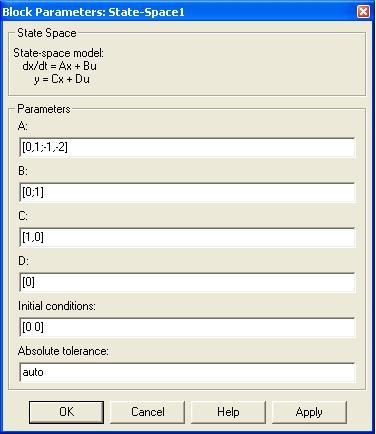
\includegraphics[width=0.6\hsize]{pix/controlandobserveentries.jpg}
                  \caption{State space configuration}\label{fig:stateConfiguration}
              \end{figure}%
              correspond to the dynamical system
              \begin{eqnarray*}
                  \dot{\vect{x}}&=&\begin{bmatrix}0&1\\-1&-2\end{bmatrix}\vect{x}
                  +\begin{bmatrix}0\\1\end{bmatrix}u,\\
                  y&=&\begin{bmatrix}1&0\end{bmatrix}\vect{x}+[0]u.
              \end{eqnarray*}
              Note that the last line specifies the initial conditions for the states.  In
              this case, we have set \(x_{1}(0)=0\) and \(x_{2}(0)=0$\@.  Come up with an
          appropriate variable to show the linear relationship between \(x_{1}\) and
          \(x_{2}\) when the system is uncontrollable (make sure you record this in your
          lab report).  Define this variable as one of your outputs in your model.
          Note that you can add as many outputs as you want just by adding rows to the
          matrix \(\vect{c}$\@.

          Define the initial conditions to be zero.  The default final time is set to
          10 by \textsf{Simulink}.  You may change it by opening the window
          \begin{center}
              \verb|Simulation|\(\rightarrow \)\verb|Configuration Parameters|
          \end{center}
          and entering the required time in the \verb|Stop Time| box.

    \item Run the \textsf{Simulink} block under uncontrollable conditions. This
          will depend on your choice of \(R_{1}\), \(R_{2}\), \(C\), and \(L\).
          Recuperate the state variable values written to the workspace and plot
          \(x_{1}\), \(x_{2}\), and the output variable you defined.  Does the output
          variable you chose show that there is, in fact, a linear relationship between
          \(x_{1}\) and \(x_{2}\)? Under these conditions, is it possible to find an input
          voltage \(E\) that will allow you to reach a point that is off this line?

    \item Add an appropriate title to your graph and print it.

    \item Rerun the system, but this time use conditions that make the system
          controllable.  Plot and print a graph of \(x_{1}\) and \(x_{2}\) and your output
          variable.  What can you now say about your output variable?  What is the set
          of reachable points under these conditions?

    \item Again, give an appropriate title to your graph and print it.
\end{enumerate}

\subsection{Observability}

When analyzing observability, you will be examining the output behaviour of
the system.  Recall that a rough definition of observability is: ``a change
in initial conditions and/or input results in a change in the output.''
\begin{enumerate}
    \item Using the work from your prelab, enter the value of \(\mat{A}\),
          \(\vect{b}\), \(\vect{c}\), and \(\mat{D}\) into the \verb|State-Space| block.
          Change the name of the output variable from \verb|simout| to \verb|I|.

    \item We will want to examine the output using many different initial
          conditions.  Build and run the system using a pair of initial conditions that
          are in the kernel of the observability matrix.  Plot, and print a graph of
          the output variable \(I$.  Make sure that you include values of the constants
          in the title of the plot.

    \item Rerun the system using a different pair of initial conditions that are
          also in the kernel of the observability matrix.  Include a plot of the
          output.  Does the result of this experiment confirm your work from the
          prelab? What happens if you use initial conditions that are not in the kernel
          of the observability matrix?
\end{enumerate}

When you have completed the lab, make sure you move the files created in the
directory created in Lab~\ref{chap:intro}.

%%% Local Variables: 
%%% mode: latex
%%% TeX-master: "lab-manual"
%%% End: 


\appendix
\chapter{Matlab}\label{chap:MATLAB}

The students of this course should be familiar with the basic ideas of
computer programming and Matlab from first year courses.

\section{Defining variables}

\begin{itemize}
\item \verb|x=3|\\
Defines the variable \verb|x| to be the constant 3.
\item \verb|x=(1,2;3,4;5,6)|\\
Defines the variable \verb|x| to be the $3 \times 2$ matrix
\begin{equation*}
\begin{bmatrix}1&2\\3&4\\5&6\end{bmatrix}
\end{equation*}
Elements of a row are delimited by commas (or spaces) and each row is
delimited by a semicolon.
\end{itemize}

\section{General Commands}

\begin{itemize}
\item \verb|dir|\\
Displays a list of files in the current directory.
\item  \verb|open lab_1.mdl|\\
Opens the specific file in the argument. We will be dealing mostly with
\verb|*.mdl| and \verb|*.m| files.
\item \verb|who|\\
Displays a list of variables in the memory of \textsf{Matlab}.
\item \verb|simulink|\\
Opens the \verb|Simulink Browser Library| window.  Using the GUI control, you
can drag and drop the blocks to build the \textsf{Simulink} models needed for
each lab.  Details on using \textsf{Simulink} and WinCon are discussed in
Appendix~\ref{chap:simulink}.
\end{itemize}

\section{Plotting}

\begin{itemize}
\item \verb|plot (lab_1_Tachometer)|\\
Plots the data from the variable \verb|lab_1_Tachometer| in \textsf{Matlab} memory.
You can check the list of variables in the \textsf{Matlab} memory by using the
\verb|who| command.

\item \verb|plot (lab_1_Tachometer,'r:')|\\
Plots the result in the memory of \textsf{Matlab} and specifies the colour of
the graph to be red and the line style to be dotted.  Colour and line format
are optional commands and they do not have to be specified for the plot
command to produce an output. You can also specify one style parameter
without the other.  The default colour is blue and the default line style is
solid.  Table~\ref{tab:colour} is a list of colours and line styles that can
be used with the plot command.
\begin{table}[htbp]
\centering
\begin{tabular}{|c|c|}\hline
Line style/colour & \textsf{Matlab} command\\\hline
solid & '\verb|-|'\\\hline
dashed &'\verb|--|'\\\hline
dotted & '\verb|:|'\\\hline
dash-dot&'\verb|-.|'\\\hline
blue & '\verb|b|' or '\verb|blue|'\\\hline
black& '\verb|k|' or '\verb|black|'\\\hline
cyan & '\verb|c|' or '\verb|cyan|' \\ \hline
green & '\verb|g|' or '\verb|green|' \\\hline
magenta & '\verb|m|' or '\verb|magenta|' \\ \hline
red & '\verb|r|' or '\verb|red|'\\ \hline
white & '\verb|w|' or '\verb|white|'\\ \hline
yellow &'\verb|y|' or '\verb|yellow|' \\ \hline
\end{tabular}
\caption{Colour commands in \textsf{Matlab}}\label{tab:colour}
\end{table}

\item \verb|title ('Angular Velocity of the Motor')|\\
Sets the title of the plot to the text in quotations.

\item \verb|xlabel ('Time (s)')|\\
Sets the x-axis label of the plot to the text in quotations.

\item \verb|ylabel ('rad/sec')|\\
Sets the y-axis label of the plot to the text in quotations.

\item \verb|hold|\\
Hold the current graph in figure and allow the user to plot more than one set
of data on the same figure.

\item \verb|hold off|\\
Release the current graph in figure and allow a new plot to replace the
current graph.
\end{itemize}

\section{Control System Toolbox}

\begin{itemize}
\item \verb|sys = ss(A,b,c,D)|\\
Defines the the state-space system from matrices $\mat{A}$\@, $\vect{b}$\@,
$\vect{c}$\@, and $\vect{D}$\@.  For a model with $n$ states and $1$ output,
\begin{itemize}
\item $\mat{A}$ is an $n\times n$ matrix,
\item $\vect{b}$ is an $n\times 1$ matrix,
\item $\vect{c}$ is a $1\times n$ matrix ($\vect{c}^{t}$ in our notation),
and
\item $\mat{D}=[0]$ (always true for this class).
\end{itemize}


\item \verb|h = tf([1 0],[1 2 10])|\\
Defines the variable \verb|h| to be the transfer function
\begin{equation*}
\frac{s}{s^{2}+2s+10}.
\end{equation*}

\item \verb|h = zpk([1 0],[-1 -2 -10],[3])|\\
Defines the variable \verb|h| to be the transfer function using the location
of the zeros, poles, and a multiplicative constant:
\begin{equation*}
\frac{3s(s-1)}{(s+1)(s+2)(s+10)}.
\end{equation*}

\item \verb|h = tf(sys)|\\
Defines the variable \verb|h| to be the transfer function for a given
state-space system.

\item \verb|sys = tf2ss[tf]|\\
Gives the SISO linear system corresponding to the transfer function \verb|tf|.

\item \verb|bode(sys)|\\
Produces the Bode plots for the given system.

\item \verb|impulse(sys)|\\
Produces the impulse response for the given system.

\item \verb|nyquist(sys)|\\
Produces the Nyquist plot for the given system.

\item \verb|margin(sys)|\\
Produces the gain and phase margins with associated crossover frequencies.
\end{itemize}

%%% Local Variables: 
%%% mode: latex
%%% TeX-master: "lab-manual"
%%% End: 

\chapter{Simulink}\label{chap:simulink}

\textsf{Simulink} allows simulation of complex control systems using a drag
and drop block diagram interface.  \textsf{Simulink} is especially useful
when used in conjunction with the Real-Time Workshop which allows
\textsf{Simulink} diagrams to be converted into C codes which can be run in
real-time on a number of so-called targets (the PC being one such target).

\section{Starting}

\begin{itemize}
\item To use \textsf{Simulink}, one must first start \textsf{Matlab}.  After
starting \textsf{Matlab}, you would type \verb|simulink| in the
\textsf{Matlab} command prompt to get the \verb|Simulink Library Browser|
window.

\item Selecting \verb|File|$\to$\verb|New|$\to$\verb|Model| (or
\verb|Ctrl+N|) while in the \verb|Simulink Library Browser| will give you a
blank model window into which you can drag-and-drop system blocks from the
\verb|Simulink Library Browser| to build a \textsf{Simulink} model.  These
models can be saved as \verb|*.mdl| files for future simulations and editing.
\end{itemize}

\section{Building a \textsf{Simulink} model}

\begin{itemize}
\item To connect the output of block~A to the input of block~B, simply
left-click the output port of block~A and drag the line that would appear
into the input port of the block~B.

\item In order to connect the output of a block into the inputs of multiple
blocks at the same time, you can right-click on an existing connection to get
another line and drag that connection into the input of another block.

\item When a block is dragged into the model window, it will be given a
generic name.  For example, when the \verb|scope| block is dragged into a
model, it would simply be labelled as ``scope'' and if it was the second
\verb|scope| block to be dragged into the model, it would be labelled as
``scope2''.  It is a good practice to rename these blocks and give them more
appropriate labels.  These names are usually suggested in the diagram of the
models in each lab. To rename a block, simply click on the existing name once
and edit.
\end{itemize}

\section{Simulations}

\begin{itemize}
\item One could view and edit the simulation parameters by clicking on
\begin{center}
\verb|Simulation|$\to$\verb|Simulation Parameters|
\end{center}
(or \verb|Ctrl+E|) while editing the model.  For the purpose of this course,
there are only three things that you have to worry about:
\begin{enumerate}
\item Start and stop time: The default start time is 0 and the default stop
time is 10.  Usually, there is no reason to change the default start time,
but you might find it useful to extend the stop time so that you could
observe the simulation for a longer period of time.

\item Solver Method: You must have this set to a fixed-step when implementing
real-time controllers. The default solver is a discrete method. You need to
change it from the default method to \verb|ode4|, which is an implementation
of the Runge-Kutta method.

\item Step size: The default setting of 0.001 corresponds to 1000 Hz sampling
frequency.  This is the fastest rate at which the system can sample.
\end{enumerate}
\end{itemize}

\section{Plotting}

\begin{itemize}
\item The outputs of a simulation can be captured by using the
\verb|To Workspace| block.  The data would be recorded as a variable in
memory of \textsf{Matlab}.  The default name of the output is \verb|simout|,
but you should change the name of this output just as you would give
appropriate label to the block itself.  One could plot the simulation output
by using plot command discussed in Appendix~\ref{chap:MATLAB}\@.
\end{itemize}

\subsection{Saving data via the ``To Workspace'' block}

This is the preferred method of saving data to your \textsf{Matlab}
workspace.  The \verb|To Workspace| block can be found at
\begin{center}
\verb|Simulink|$\to$\verb|Sinks|
\end{center}
Drag this block into your workspace and connect it to the variable you wish
to save.  Double click on the block to configure it.  Choose a good variable
name and in the \verb|save format| drop down menu select
\verb|Structure with time|.  After the simulation the data will be
automatically saved to your \textsf{Matlab} workspace and you can plot it
with the command
\begin{center}
\verb|plot(varname.time,varname.signals.values)|
\end{center}
replacing ``\verb|varname|'' with the variable name you chose when
configuring the \verb|To Workspace| block.

\subsection{Saving data from a scope}

You can also save scope data, but the scope seems to have short-term memory
loss which makes it one of the most useless blocks in the simulink library.
Nevertheless if you need to save the data from a scope, follow these
instructions.
\begin{enumerate}
\item Double click on the scope you wish to save the data from.
\item Click on the Parameters Icon (in the top left of the scope dialog box).
\item Data History Tab
\begin{itemize}
\item Uncheck box \verb|Limit data points|
\item Check box \verb|Save data to workspace|
\item Choose a variable name
\item Select \verb|Array| from the Format drop down menu.
\end{itemize}
\item Click \verb|Apply| and \verb|OK| to exit.
\end{enumerate}
After the simulation has been performed, the data will appear as an array in
your \textsf{Matlab} workspace.  You can plot the data with the
command \begin{center}
\verb|plot(ScopeData1(:,1), ScopeData1(:,2))|
\end{center}
where \verb|ScopeData1| is the variable name that you set in the above steps.

%%% Local Variables: 
%%% mode: latex
%%% TeX-master: "lab-manual"
%%% End: 

\chapter{Lab Equipment}\label{chap:hardware}

In the lab, there are several computers equipped with data acquisition
systems running Windows~7 with Matlab. The hardware equipment and some
software tools are manufactured by \href{http://www.quanser.com/}{Quanser
    Consulting}, a Canadian company developing real-time control systems for
education and research. This document introduces some of the hardware
equipment to be used in the labs. Familiarity with this document is needed to
perform the labs.

\section{Servomotor (Lab 1)}
\subsection{Hardware devices}

The lab hardware consists of three components:
\begin{enumerate}
    \item data acquisition system;
    \item power module;
    \item servomotors.
\end{enumerate}

\subsection{Data Acquisition Board}

In order for the computer to run a controller, analog-to-digital (A/D) and
digital-to-analog (D/A) conversions are necessary. These are done using the
data acquisition and control board (DACB), which inputs the measured
signal(s) to the computer and outputs control action to the actuator in the %chktex 36
control loop.  The DACB in this lab consists of a single board: the Q2-USB,
which is made by Quanser Consulting.  Figure~\ref{fig:q2usb}
\begin{figure}[htbp]
    \centering
    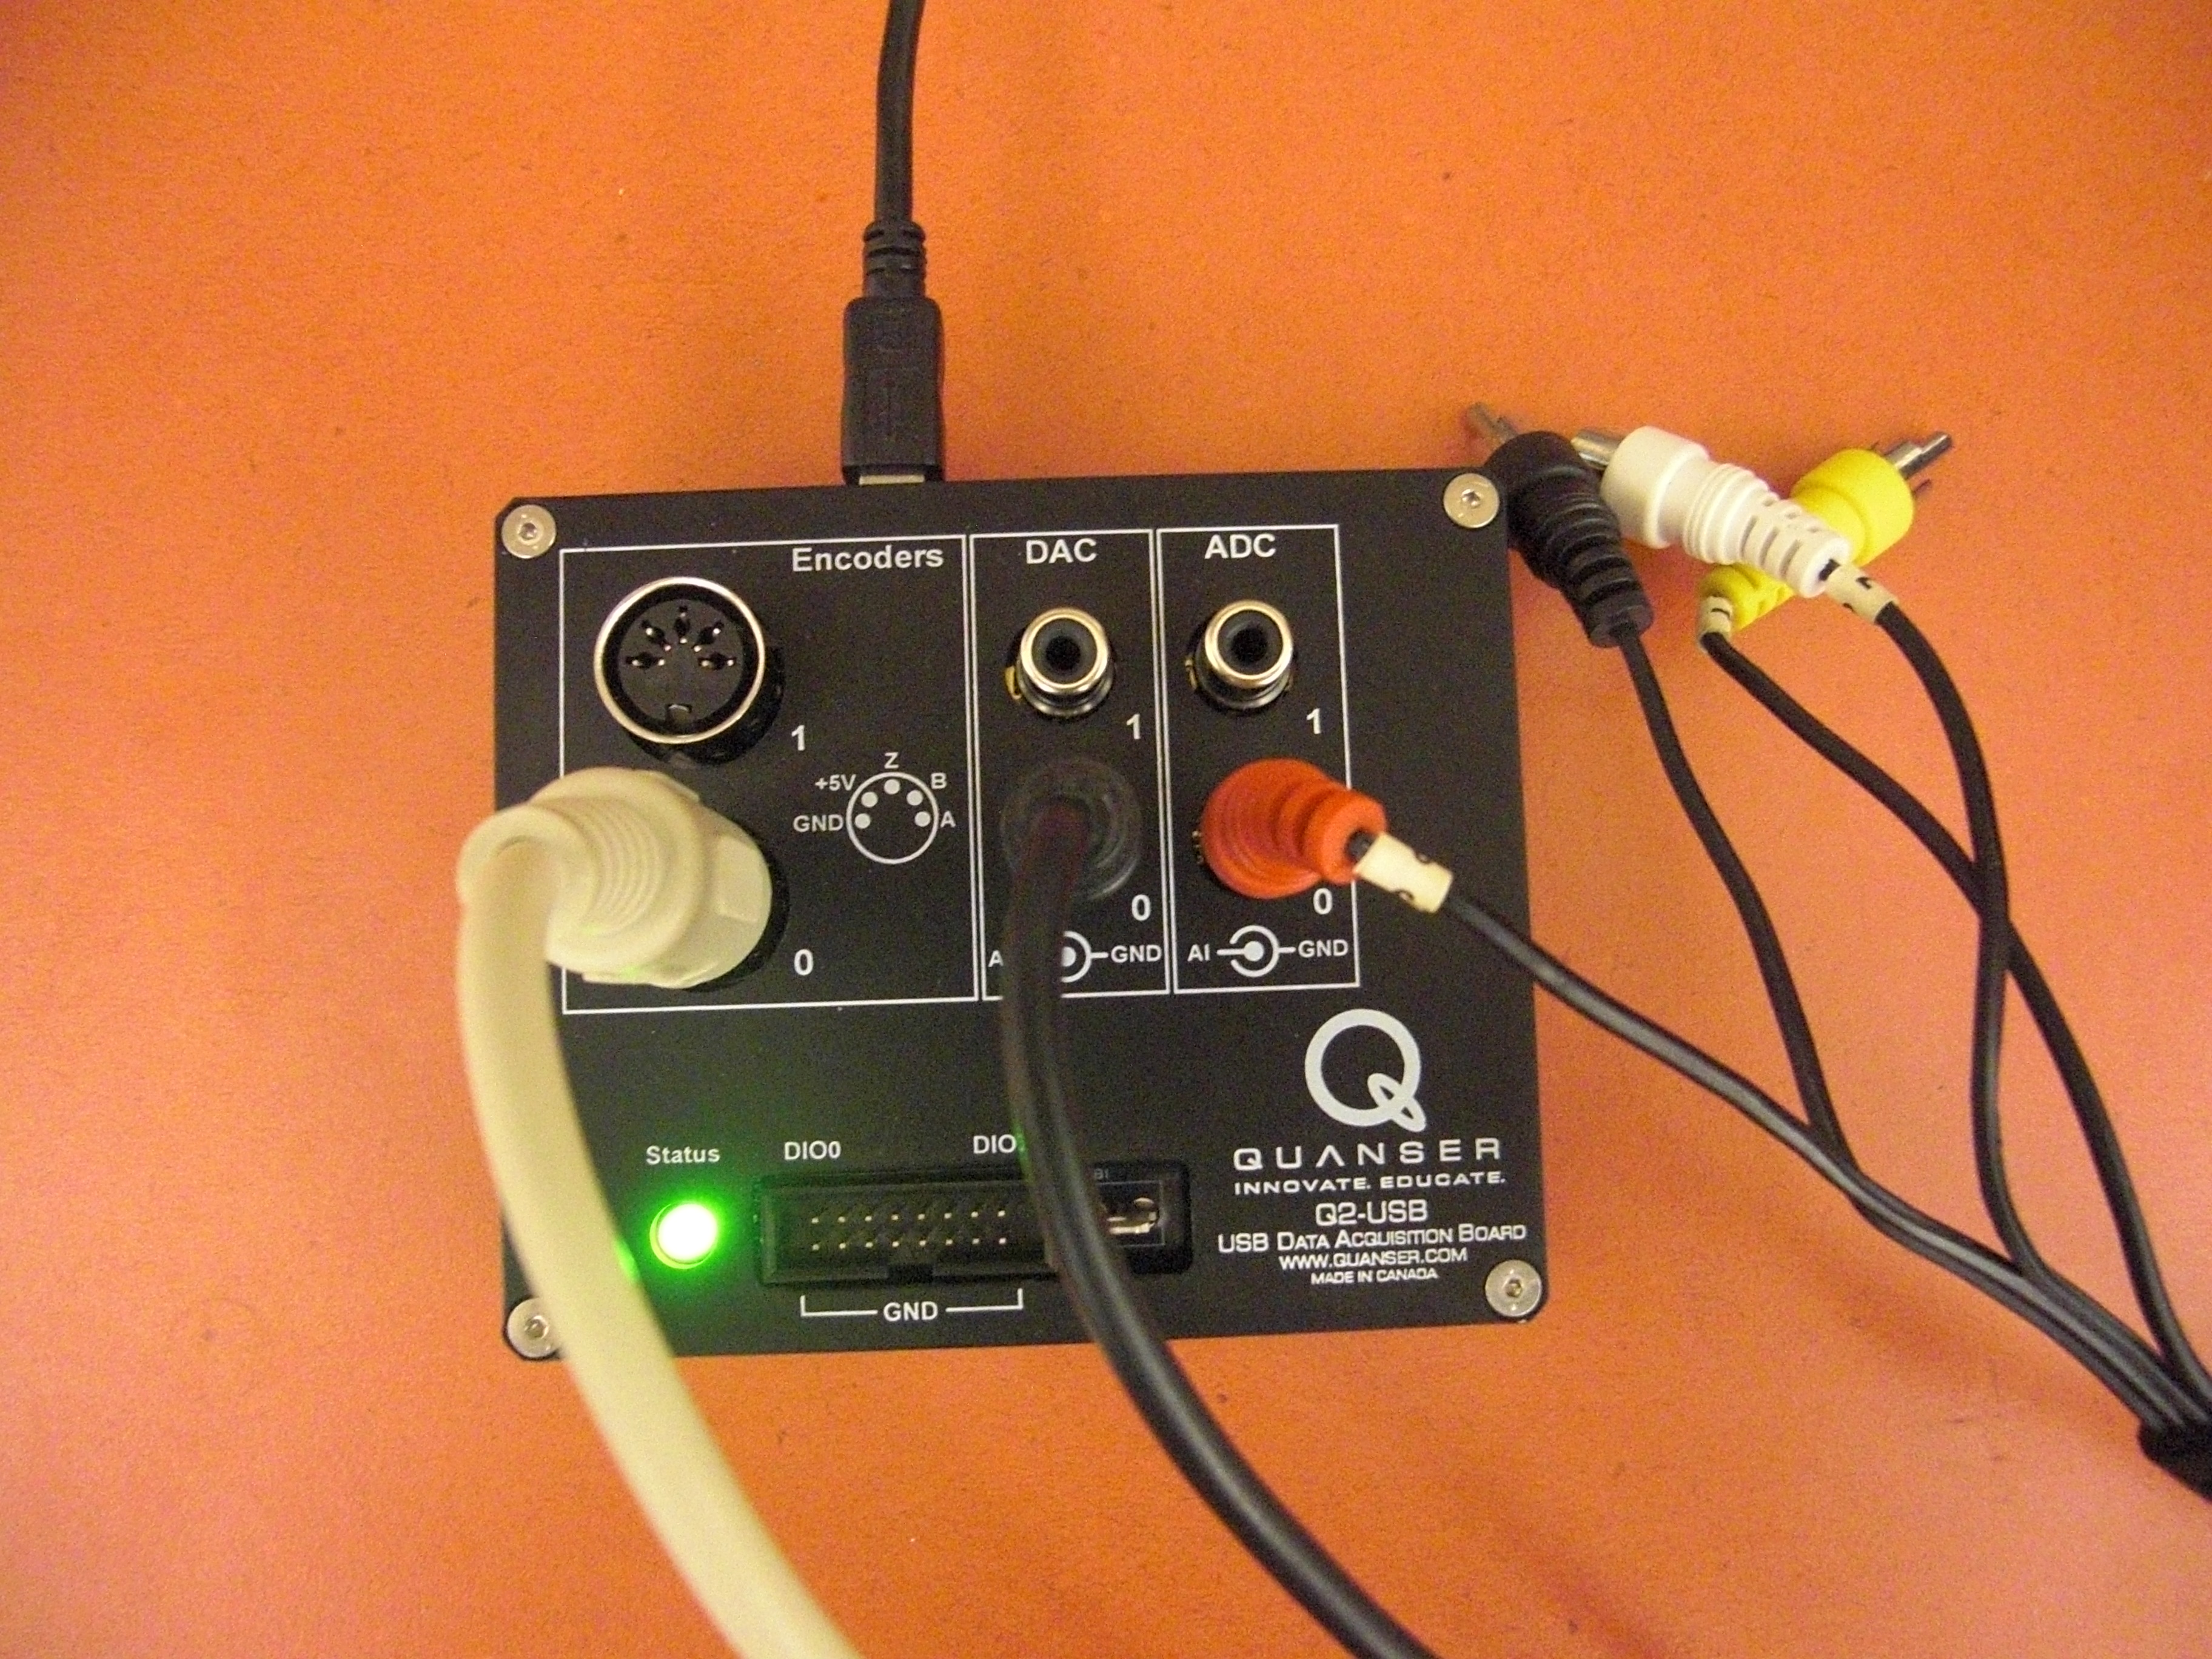
\includegraphics[width=0.6\hsize]{pix/Q2USB.jpg}
    \caption{Q2-USB data acquisition board}\label{fig:q2usb}
\end{figure}%
shows a photo of the Q2-USB card. This data acquisition board is an external
board connected to the computer through a USB port.

Figure~\ref{fig:q2usb} also shows the proper configuration of the data
acquisition board.  The Encoder is the 5~pin Din and is plugged in to
channel~0 in the Encoders portion of the board. The tachometer (S3 on the
Quanser) is the red RCA plug and is plugged into channel~0 is the ADC
portion of the board.  Finally the analog output is the solo black RCA plug
and is plugged in to channel~0 of the DAC portion of the board.

\subsection{Universal power module}

The universal power module (UPM-2405), which is shown in
Figure~\ref{fig:power}\@,
\begin{figure}[htbp]
    \centering
    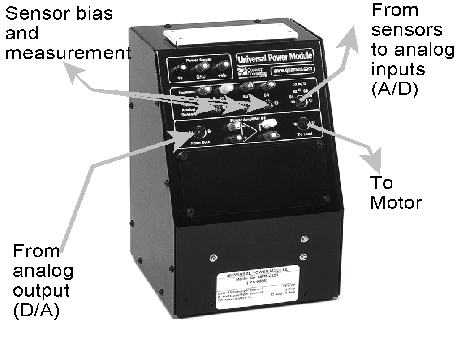
\includegraphics[width=0.6\hsize]{pix/power.jpg}
    \caption{Universal power module}\label{fig:power}
\end{figure}%
is a linear power operations amplifier. The Q2-USB data acquisition board
cannot deliver enough power to the actuators used in this lab; therefore, a
signal buffer is needed.  The UPM-2405 is used as our signal buffer since it
can deliver up to 5A~to an actuator in a non-inverting, unity gain
configuration.

The following connections can be made to/from the UPM (see the labels on the
UPM).
\begin{itemize}
    \item From analog sensors: there are four (S1-S4 inputs which can be
          connected from analog sensors (and then subsequently to the computer); the
          cable used is a 6-pin mini-din/6-pin mini-din cable (light tan colour), which
          is now referred to as the analog sensor cable.

    \item To A/D:\@ the four analog sensor signals (S1-S4) can then be connected to
          the Q2-USB terminal board for A/D conversion into the computer; the cable
          used is a 5-pin din-stereo/4RCA cable (black colour), which is now referred to
          as the A/D cables.

    \item From D/A:/@ this is where you input the D/A signal from the Q2-USB
          terminal board to the UPM;\@ the cable used is a 5-pin din-mono/RCA cable
          (black colour), which is now referred to as the D/A cable.

    \item To load: here you connect the amplified D/A signal to an actuator
          (e.g., servomotor); the cable used is a 7-pin din/4-pin din cable (black
          colour), which is now referred to as the load cable.  Note there are two types
          of load cables one with unity gain and another with a cable gain of 5.  Make
          sure you use the right one.

    \item Others: A few other connections are possible for convenience: e.g., a
          DC power supply on the top left provides 12 volts; the signal s from analog
          sensors S1-S4 can be easily monitored by connecting to a scope to the banana
          plug terminals.
\end{itemize}

\subsection{DC servomotor}

The Quanser DC servomotor (SRV02) is shown in Figure~\ref{fig:motor}\@.  A 3W
motor is mounted in a solid aluminium frame and drives a built-in Swiss-made
14.1:1 gearbox whose output drives an external gear, which is attached to an
independent output shaft that rotates in an aluminium ball-bearing block.
The output shaft is equipped with an encoder.  The external gear on the
output shaft drives an anti-backlash gear connected to a precision
potentiometer for measuring the output angle.  The external gear ratio can be
changed from 1:1 to 5:1 using different gears.  Two inertial loads are
supplied with the system in order to examine the effect of changing inertia
on motor performance.
\begin{figure}[htbp]
    \centering
    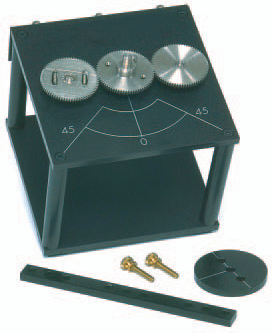
\includegraphics[width=0.6\hsize]{pix/motor-eps-converted-to.pdf}
    \caption{DC servomotor (SRV02)}\label{fig:motor}
\end{figure}%
Several connections are available for the servomotor. The input voltage
connects to the UPM using the load cable.  The potentiometer and tachometer
ports connect to the UPM-2405 using sensor cables and are used to measure
angular position and angular velocity respectively.  Additionally, the shaft
encoder port connects to the terminal board using an encoder cable and is
used to measure angular position.  The calibration factors listed in
Table~\ref{tab:conversionFactors} are needed in order to use the sensors in
units of degrees or radians.

\begin{table}[htbp]
    \centering
    \begin{tabular}{c c c }
        Connection    & Conversion (Rad)                                    & Conversion (Deg)                                   \\\bottomrule
        Encoder       & \(-\frac{2\pi}{4096}\)                              & \(-\frac{360}{4096}\)                              \\
        Tachometer    & \(\frac{100\pi}{63} \frac{\text{rad}}{\text{sec}}\) & \(\frac{18000}{63} \frac{\text{deg}}{\text{sec}}\) \\
        Potentiometer & \(\frac{1}{4096}\)                                  & \(\frac{180}{4096\pi}\)                            \\
    \end{tabular}
    \caption{Conversion factors}\label{tab:conversionFactors}
\end{table}

\section{Rotary Pendulum (Lab 3)}
\subsection{Setting up the Rotary Pendulum}\label{subsection:lab2_setup}
First, let us assemble and wire the physical system. Examine the close-up assembly shown in Figure~\ref{fig:lab1a_assembly}, and replicate this at your workstation. Note that the high-gear configuration is used here. Use the wiring diagram shown in Figure~\ref{fig:lab1a_wiring} to connect the rotary pendulum to a power source and the data acquisition board.
\begin{figure}[htb!]
    \centering
    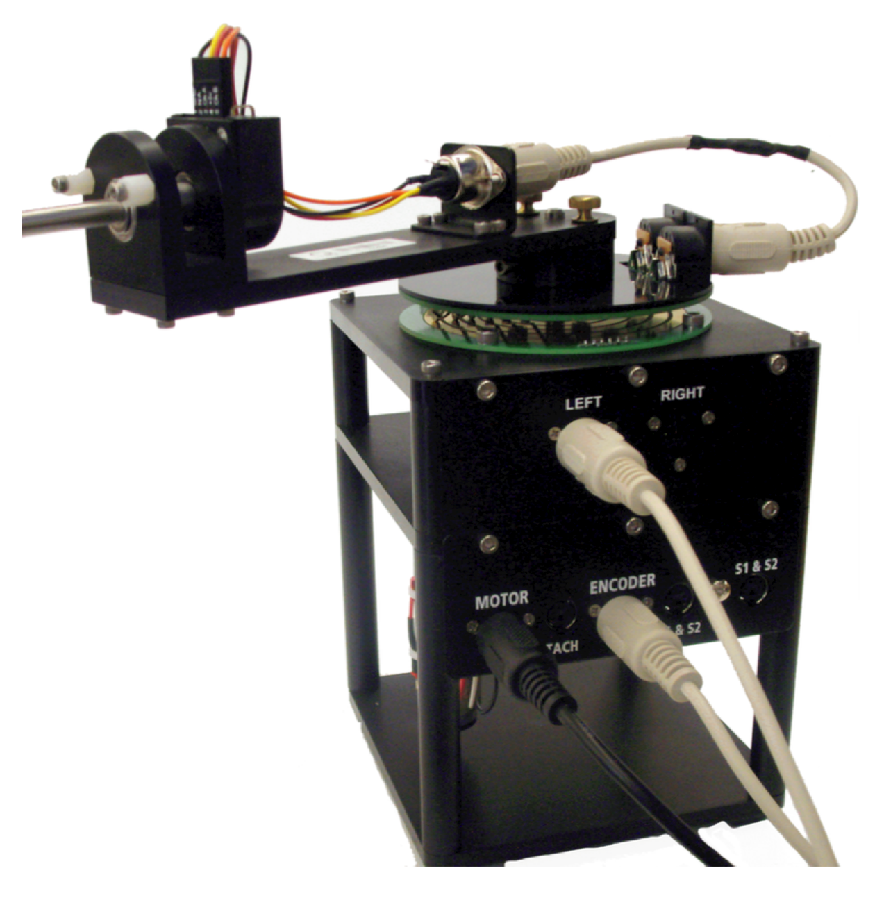
\includegraphics[width=.3\linewidth]{eps/lab_2/assembly.eps}
    \caption{A close-up of the assembly of the rotary pendulum module and the Quanser SRV02 plant~\cite{Q-Flex-Beam}.}
    \label{fig:lab1a_assembly}
\end{figure}
\begin{figure}[htb!]
    \centering
    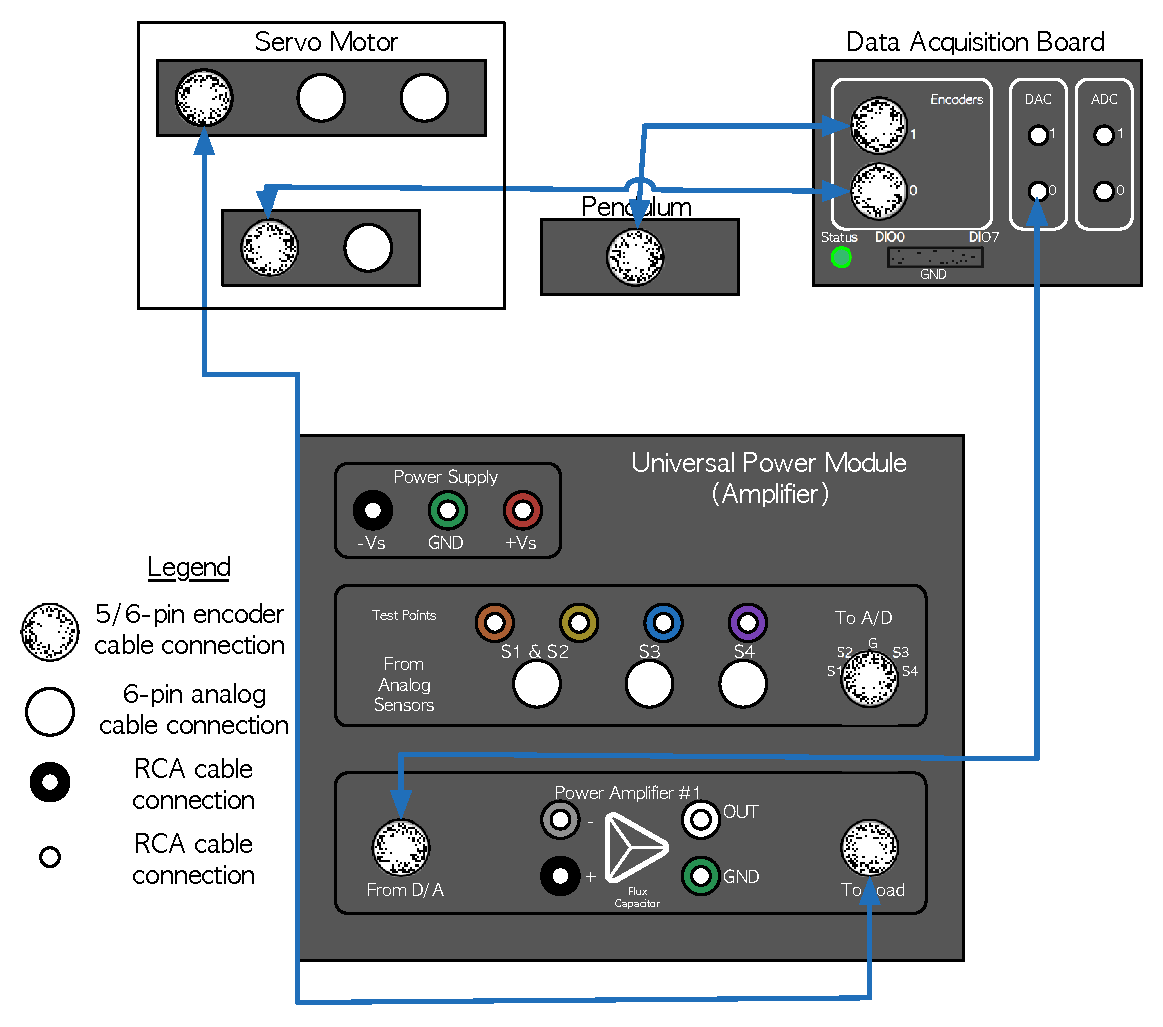
\includegraphics[width=.7\linewidth]{eps/lab_2/wiring.eps}
    \caption{A wiring diagram for the Quanser SRV02 and rotary pendulum module.}
    \label{fig:lab1a_wiring}
\end{figure}

\textbf{Note:} The power amplifier must be turned on before you can experiment with the physical system. The power switch is located at the back of the amplifier (good luck finding it). Make sure to turn off the power amplifier before you leave the lab.

\section{Flexible Beam {Lab 4}}
First, you must assemble and wire the physical system correctly. Examine the close-up assembly shown in Figure~\ref{fig:lab1_assembly} and replicate this at your workstation. Note that the high-gear configuration is used here: a large gear is connected to a small pinion and a slip gear, rather than using the smaller gear. You will need to build a two-tiered gear train as shown in Figure~\ref{fig:lab1_assembly} to make the large gear fit correctly. Use the wiring diagram shown in Figure~\ref{fig:lab1_wiring} to connect the rotary pendulum to a power source and the data acquisition board.
\begin{figure}[htb!]
    \centering
    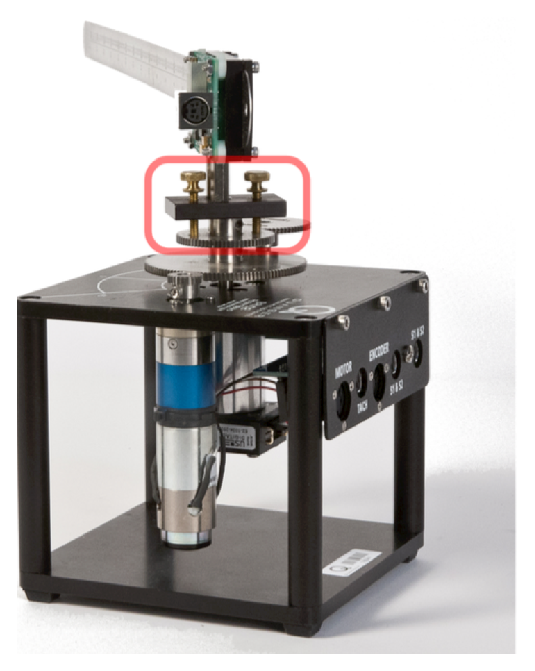
\includegraphics[width=.3\linewidth]{eps/lab_1/assembly.eps}
    \caption{A close-up of the assembly of the rotary flexible beam module and the Quanser SRV02 plant~\cite{Q-Flex-Beam}. The high-gear gear train is indicated by a red box.}
    \label{fig:lab1_assembly}
\end{figure}
\begin{figure}[htb!]
    \centering
    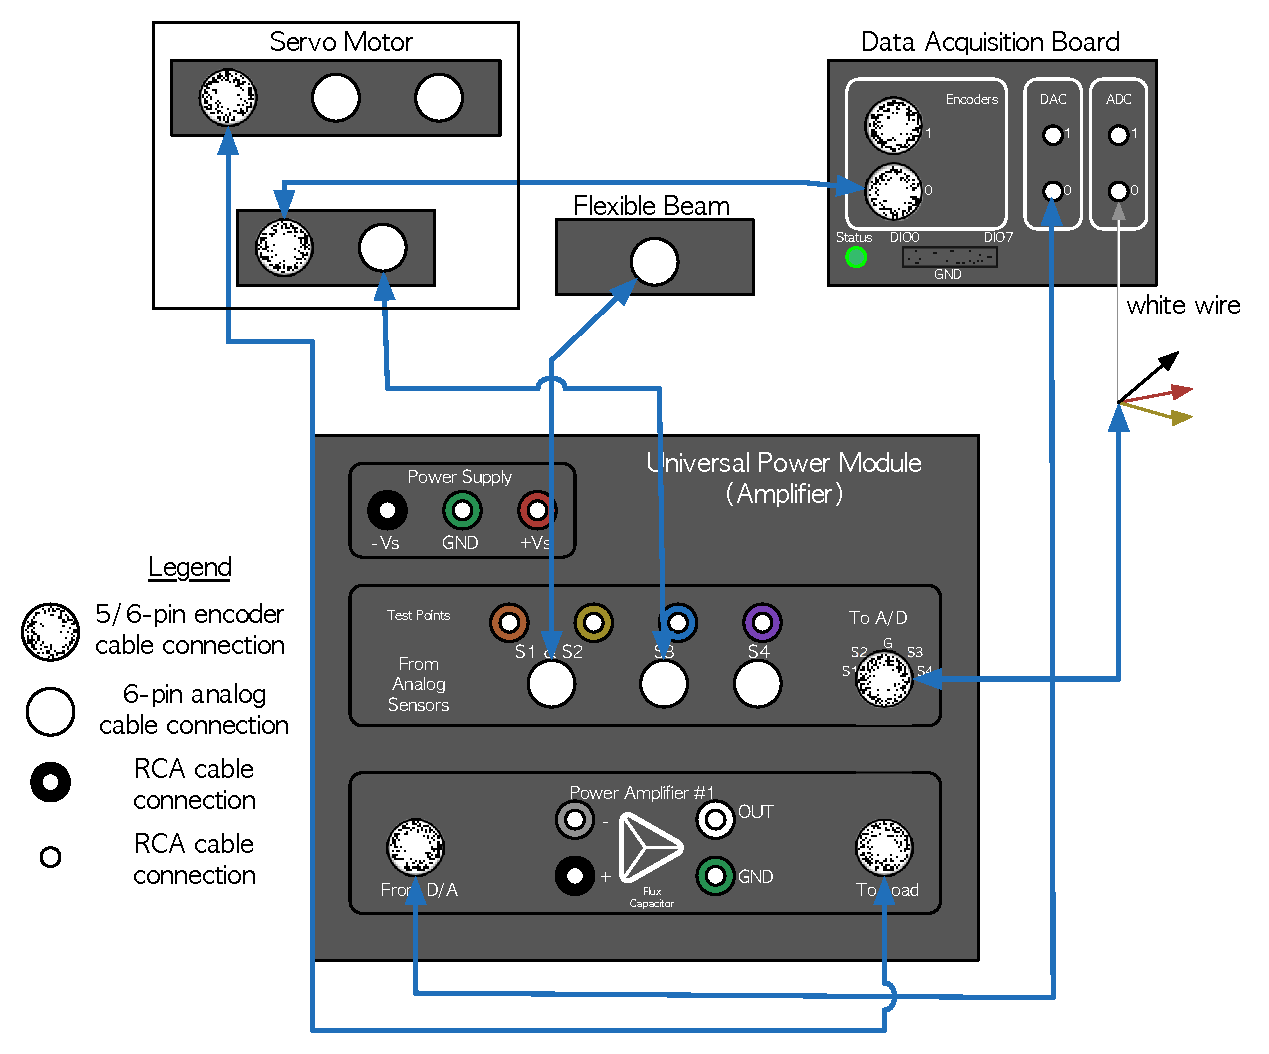
\includegraphics[width=.8\linewidth]{eps/lab_1/wiring.eps}
    \caption{A wiring diagram for the Quanser SRV02 and rotary flexible beam module.}
    \label{fig:lab1_wiring}
\end{figure}

%%% Local Variables: 
%%% mode: latex
%%% TeX-master: "lab-manual"
%%% End: 


\end{document} %chktex 17